%%%%%%%%%%%%%%%%%%%%%%%%%%%%%%%%%%%%%%%%%%%%%%%%%%%%%%%%%%%%
\documentclass[a4paper,11pt,oneside]{article}
\usepackage[a4paper,vmargin={1.5cm,1.5cm},width=16cm]{geometry}
\usepackage[style=verbose-inote,doi=false,sortcites=true,block=space,backend=bibtex]{biblatex}
\usepackage[utf8]{inputenc}
\usepackage{textcomp}
\usepackage[spanish]{babel}
\usepackage{microtype}
\usepackage{lmodern}
\usepackage{graphicx}
\usepackage{fancyhdr}
\usepackage{booktabs}
\usepackage{eurosym}
\usepackage{mathptmx}
\usepackage[T1]{fontenc}
\usepackage{hyperref}
%% Added to help mimic structure.
\usepackage[many]{tcolorbox}
\usepackage{soul}
\usepackage{color}
\usepackage{lastpage}
%\usepackage[skins]{tcolorbox}
%%%%%%%%%%%%%%%%%%%%%%%%%%%%%%%%%%%%%%%%%%%%%%%%%%%%%%%%%%%%
%% HEADERS
%\setlength{\headheight}{1cm}
%\setlength{\headsep}{0.5cm}
%\pagestyle{fancyplain}
%\fancyhf{}
%\lhead{\fancyplain{}{\sc Memoria científico técnica de proyectos coordinados}}
%\rhead{\fancyplain{}{\sc Parte A}}
%\cfoot{\thepage}
%\renewcommand{\headrulewidth}{0pt} % remove lines
%\renewcommand{\footrulewidth}{0pt}


%%% HEADER
\setlength{\headheight}{1cm}
%\setlength{\headwidth}{20cm}
\setlength{\headsep}{0.5cm}
\pagestyle{fancyplain}
\fancyheadoffset[HR,HL]{2cm}
\fancyhf{}
\lhead{\raisebox{-0.4\height}{
\includegraphics[height=0.9cm,keepaspectratio=true]{img/miniLogo}}}
\rhead{\fancyplain{}{\fontsize{10}{12} \selectfont \textbf{\underline{Memoria científico técnica de proyectos coordinados}}}}
\cfoot{\thepage\, / parte A}
\renewcommand{\headrulewidth}{0pt} % remove lines
\renewcommand{\footrulewidth}{0pt}
%%%%%%%%%%%%%%%%%%%%%%%%%%%%%%%%%%%%%%%%%%%%%%%%%%%%%%%%%%%%
%% Hack to make math formulas bold in section titles
\makeatletter
\DeclareRobustCommand*{\bfseries}{%
  \not@math@alphabet\bfseries\mathbf
  \fontseries\bfdefault\selectfont
  \boldmath
}
\makeatother

%%%%%%%%%%%%%%%%%%%%%%%%%%%%%%%%%%%%%%%%%%%%%%%%%%%%%%%%%%%%
\def\thesection{\bf \textsf{\Alph{section}}}

%\nobibliography{biblio}
%\bibliographystyle{JHEP}

\bibliography{biblio}


%%%%%%%%%%%%%%%%%%%%%%%%%%%%%%%%%%%%%%%%%%%%%%%%%%%%%%%%%%%%
\begin{document}

%% Some useful definitions
% BB
\newcommand{\bb}{\ensuremath{\beta\beta}}
% BB0NU
\newcommand{\bbonu}{\ensuremath{\beta\beta0\nu}}
% BB2NU
\newcommand{\bbtnu}{\ensuremath{\beta\beta2\nu}}
% NME
\newcommand{\Monu}{\ensuremath{\Big|M_{0\nu}\Big|}}
\newcommand{\Mtnu}{\ensuremath{\Big|M_{2\nu}\Big|}}
% PHASE-SPACE FACTOR
\newcommand{\Gonu}{\ensuremath{G_{0\nu}(\Qbb, Z)}}
\newcommand{\Gtnu}{\ensuremath{G_{2\nu}(\Qbb, Z)}}

% mbb
\newcommand{\mbb}{\ensuremath{m_{\beta\beta}}}
\newcommand{\kgy}{\ensuremath{\rm kg \cdot y}}
\newcommand{\ckky}{\ensuremath{\rm counts/(keV \cdot kg \cdot yr)}}
\newcommand{\mbba}{\ensuremath{m_{\beta\beta}^a}}
\newcommand{\mbbb}{\ensuremath{m_{\beta\beta}^b}}
\newcommand{\mbbt}{\ensuremath{m_{\beta\beta}^t}}
\newcommand{\nbb}{\ensuremath{N_{\beta\beta^{0\nu}}}}

% Qbb
\newcommand{\Qbb}{\ensuremath{Q_{\beta\beta}}}

% Tonu
\newcommand{\Tonu}{\ensuremath{T_{1/2}^{0\nu}}}

% Tonu
\newcommand{\Ttnu}{\ensuremath{T_{1/2}^{2\nu}}}

% Xe-136
\newcommand{\Xe}{\ensuremath{^{136}}Xe}

% 2S
\newcommand{\TwoS}{\ensuremath{^{2}S_{1/2}}}

\newcommand{\TwoP}{\ensuremath{^{2}P_{1/2}}}

\newcommand{\TwoD}{\ensuremath{^{2}D_{3/2}}}


% Xe-136
\newcommand{\CS}{\ensuremath{^{137}}Cs}

% Xe-136
\newcommand{\NA}{\ensuremath{^{22}}Na}


% Bi-214
\newcommand{\Bi}{\ensuremath{^{214}}Bi}

% Tl-208
\newcommand{\Tl}{\ensuremath{^{208}}Tl}

% Pb-208
\newcommand{\Pb}{\ensuremath{^{208}}Pb}
% Pb-208
\newcommand{\PBD}{\ensuremath{^{210}}Pb}

% Po-214
\newcommand{\Po}{\ensuremath{^{214}}Po}

% bru
\newcommand{\bru}{cts/(keV$\cdot$kg$\cdot$y)}
\newcommand{\HPXE}{\sc{HPXe}\rm}
\newcommand{\BATA}{\sc{BaTa}\rm}

% Saltos de carro en tablas
\newcommand{\minitab}[2][l]{\begin{tabular}{#1}#2\end{tabular}}

\newcommand{\thedraft}{0.1.1}% version for referees

\newcommand{\MO}{\ensuremath{{}^{100}{\rm Mo}}}
\newcommand{\SE}{\ensuremath{{}^{82}{\rm Se}}}
\newcommand{\ZR}{\ensuremath{{}^{96}{\rm Zr}}}
\newcommand{\KR}{\ensuremath{{}^{82}{\rm Kr}}}
\newcommand{\ND}{\ensuremath{{}^{150}{\rm Nd}}}
\newcommand{\XE}{\ensuremath{{}^{136}\rm Xe}}
\newcommand{\GE}{\ensuremath{{}^{76}\rm Ge}}
\newcommand{\GES}{\ensuremath{{}^{68}\rm Ge}}
\newcommand{\TE}{\ensuremath{{}^{128}\rm Te}}
\newcommand{\TEX}{\ensuremath{{}^{130}\rm Te}}
\newcommand{\TL}{\ensuremath{{}^{208}\rm{Tl}}}
\newcommand{\CA}{\ensuremath{{}^{48}\rm Ca}}
\newcommand{\CO}{\ensuremath{{}^{60}\rm Co}}
\newcommand{\PO}{\ensuremath{{}^{214\rm Po}}}
\newcommand{\U}{\ensuremath{{}^{235}\rm U}}
\newcommand{\CT}{\ensuremath{{}^{10}\rm C}}
\newcommand{\BE}{\ensuremath{{}^{11}\rm Be}}
\newcommand{\BO}{\ensuremath{{}^{8}\rm Be}}
\newcommand{\UDTO}{\ensuremath{{}^{238}\rm U}}
\newcommand{\CD}{\ensuremath{^{116}{\rm Cd}}}
\newcommand{\THO}{\ensuremath{{}^{232}{\rm Th}}}
\newcommand{\BI}{\ensuremath{{}^{214}}Bi}


%% Heading
\begin{tcolorbox}[colback=white,arc=0pt,outer arc=0pt,colframe=black,boxrule=0.6pt]
\begin{center}
Convocatorias 2016\\ 
Proyectos Excelencia y Proyectos RETOS \\ 
Dirección General de Investigación Científica y Técnica \\
Subdirección General de Proyectos de Investigación
\end{center} 
\end{tcolorbox}

\begin{tcolorbox}[colback=yellow,arc=0pt,outer arc=0pt,colframe=black,boxrule=0.6pt,left=0mm,right=0mm]
  \begin{center}
    AVISO IMPORTANTE\\
  \end{center}
    En virtud del art\'iculo 11 de la convocatoria \ul{\textbf{NO SE ACEPTAR\'AN NI SER\'AN SUBSABABLES MEMORIAS CIENT\'IFICO-T\'ECNICAS}} que no se presenten en este formato.
     \\
    \textbf{La parte C no podrá exceder 25 p\'aginas.}
    \\
    \\
    \textbf{Lea detenidamente las instrucciones para rellenar correctamente esta memoria disponibles en la web de la convocatoria .}
    \\
  %\end{center}
\end{tcolorbox}
\vspace{3pt}
\begin{tcolorbox}[colback=yellow,arc=0pt,outer arc=0pt,colframe=black,boxrule=0.6pt,left=0mm]
  \noindent\textbf{Parte A: RESUMEN DE LA PROPUESTA/SUMMARY OF THE PROPOSAL}
  %\section{RESUMEN DE LA PROPUESTA/SUMMARY OF THE PROPOSAL}
\end{tcolorbox}

%%%%%%%%%%%%%%%%%%%%%%%%%%%%%%%%%%%%%%%%%%%%%%%%%%%%%%%%%%%%%%%%%%%%%%%%%%%%%

%\section{RESUMEN DE LA PROPUESTA/SUMMARY OF THE PROPOSAL}

%%%%%%%%%%%%%%%%%%%%%%%%%%%%%%%%%%%%%%%%%%%%%%%%%%%%%%%%%%%%%%%%%%%%%%%%%%%%%

%\subsection{DATOS DEL PROYECTO COORDINADO}
\noindent\textbf{A.1. DATOS DEL PROYECTO COORDINADO}
\vspace{6pt}

\noindent\textbf{INVESTIGADOR COORDINADOR PRINCIPAL 1:} (Nombre y apellidos)

\noindent José Díaz Medina.
\vspace{6pt}

\noindent\textbf{INVESTIGADOR COORDINADOR PRINCIPAL 2:} (Nombre y apellidos)

\noindent 
\vspace{6pt}

\noindent\textbf{TÍTULO GENERAL DEL PROYECTO COORDINADO:} Desarrollo de un nuevo tipo de aparato PET de alta sensibilidad basado en xenón líquido.
\vspace{6pt}

\noindent\textbf{ACRÓNIMO DEL PROYECTO COORDINADO:} PETALO.


\noindent\textbf{RESUMEN DEL PROYECTO COORDINADO} 
{\color{blue}{M\'aximo 3500 caracteres (incluyendo espacios en blanco):}}
\vspace{12pt}

El xenón es un gas noble, que centellea en respuesta a la radiación ionizante. La señal de centelleo del xenón líquido es muy rápida y muy intensa, siendo por tanto potencialmente útil para la imagen médica.

Este proyecto se desarrollará en dos fases concurrentes. En primer lugar, se realizará una investigación 
exhaustiva de la física del xenón líquido (LXe de sus siglas en inglés) y se caracterizarán las prestaciones de un nuevo tipo de celda de detección, llamada la Celda Centelleante de Xenón Líquido (LXSC), cuyo diseño básico es el de una caja llena con LXe y leída por fotomultiplicadores de silicio (SiPMs). Recientes estudios de
Monte Carlo indican que la LXSC puede conseguir una excelente resolución espacial y de energía, al igual que un tiempo de coincidencia (``coincidence resolving time'', o CRT) muy bueno. Estas capacidades serán estudiadas
experimentalmente durante la primera fase del proyecto, usando un dispositivo experimental denominado P2. El mismo dispositivo será también utilizado para estudiar las prestaciones de nuevos detectores y electrónica muy rápidos, con la posible aplicación de la detección de la luz de Cherenkov and LXe. Esta actividad se realizará en estrecha colaboración con el proyecto CLUES, que también se ha presentado a esta convocatoria. 

La segunda fase de este proyecto propone la construcción, puesta a punto y operación de un prototipo de un nuevo tipo de aparato PET denominado PETALO (Positron Electron TOF Apparatus using Liquid xenOn) basado en la LXSC. Las excelentes prestaciones de la LXSC hacen posible un PET de gran resolución en energía (12--14\% FWHM), buena resolución espacial (del orden de 2 mm FWHM {\em en las tres coordenadas}) y excelente resolución temporal, con un CRT de unos 100 ps. Además, el LXe es un medio continuo, lo que permite diseñar un detector muy compacto en el que se minimizan las áreas ciegas. La operación criogénica de los SiPMs permite eliminar completamente una de las fuentes de ruido más importantes de estos detectors, la corriente oscura. Por último, el coste del xenón líquido es muy inferior al LYSO (3 \euro/cc, a comparar con 40-50 \euro/cc). Todos estos factores se combinan para ofrecer la posibilidad de construir un detector de gran tamaño y alta sensibilidad (``PET de cuerpo completo'', con una longitud axial del orden de cinco veces la de los actuales dispositivos) basado en el LXe, con excelentes prestaciones para tiempo de vuelo (TOF).  

Este proyecto coordina tres grupos cuya experiencia combinada permiten la construcción y puesta a punto del prototipo mencionado,  llamado PEP (PEtalo Prototype). El subproyecto DET (IFIC) está a cargo de la construcción del aparato. así como de la construcción de P2.  El subproyecto IMG (GIBI239/LaFe) está a cargo del análisis de imagen y la operación y certificación de PEP en entorno clínico. EL proyecto CLUES está liderado por el grupo ICCUB (Instituto de Ciencias del Cosmos,UB).




 
\vspace{12pt}

\noindent\textbf{PALABRAS CLAVE DEL PROYECTO COORDINADO:} PET, xenón líquido, TOF, SiPM, centelleo, sensibilidad, CRT.
\vspace{12pt}

\noindent\textbf{TITLE OF THE COORDINATED PROJECT:} Development of a new PET apparatus of high sensitivity based on liquid xenon
\vspace{6pt}

\noindent\textbf{ACRONYM OF THE COORDINATED PROJECT:} PETALO.
\vspace{6pt}

\noindent\textbf{SUMMARY OF THE COORDINATED PROJECT} 
\vspace{6pt}

This project proposes a proof-of-concept for a new type of PET apparatus, called
PETALO (Positron Electron TOF Apparatus using Liquid xenOn). The active target is liquid xenon (LXe), read by silicon photomultipliers (SiPMs). The basic element of PETALO is the Liquid Xenon Scintillating Cell (LXSC). The simplest design of such a cell is a box in which one of its faces (the exit face w.r.t. the fly direction of the gammas) is instrumented, while the other faces are covered with reflecting Teflon sheets. The best ratio in cost to performance is obtained with the LXSC2, which instruments  the entry and exit faces of the box, achieving excellent energy resolution and spatial resolution (in the three coordinates), as well as superb coincidence resolving time (CRT).  

Xenon is a noble gas which scintillates as response to the ionising radiation. The scintillation is very fast (it is mediated by two constants, una of 2.2 ns and the other one of 27 ns) and very intense (30,000 photons per 511 keV gamma). The combination of both features results in the possibility of building a PET of excellent energy resolution (better than 12-14\% FWHM, which is the same order as the top-of-the-line present LYSO scanners), very good spatial resolution
(of the order of 2 mm FWHM {\em in the three coordinates})  and excellent time resolution, with a CRT of about 100 ps. Furthermore, LXe is a continuous medium, allowing a very compact detector, with minimal dead areas. Cryogenic operation of SiPMs, on the other hand, permits suppressing to negligible levels one of the most important noise sources of this type of sensors (dark current). Last, but not least, xenon is much cheaper than LYSO (3 \euro/cc to be compared with 40--50 \euro/cc). All this factors put together result in the possibility of using the technology to build a large PET scanner of competitive cost and high sensitivity (``full body PET, with an axial length at least 5 times larger than current devices), based in LXe, with excellent TOF capabilities. The use of time of flight to reduce imaging errors is known since the beginning of the technology and the last few years have witnessed a rekindled interest in the technique, including the introduction in the market of a commercial model boasting a CRT of 600 ps (the GEMINI, manufactured by Philips). Other recent devices feature improved CRT near 400 ps. PETALO could achieve a CRT in the range of 100 ps, thus representing a break-through in the technology.  

This projects coordinates three groups whose combined experience permits the construction and commissioning of a demonstrator of PETALO called PEP (PEtalo Prototype). The DET subproject (IFIC) is in charge of the construction  of the detector. It is also in charge of the development of the simulation and software framework, and will lead the study of PETALO as a TOF device. The ASIC subproject (I3M/UPV) is in charge of sensors, front-end electronics and DAQ. The subproject IMG 
(GIBI239/LaFe) is in charge of image analysis, as well as operation and certification of PEP in a clinical environment.   





 \vspace{12pt}

\noindent\textbf{KEYWORDS OF THE COORDINATED PROJECT:} PET, scintillation, liquid xenon, SiPMs, sensitivity, TOF, CRT.  

 \vspace{12pt}
%\newpage

%%%%%%%%%%%%%%%%%%%%%%%%%%%%%%%%%%%%%%%%%%%%%%%%%%%%%%%%%%%%%%%%%%%%%%%%%%%%%

\noindent\textbf{A.2. DATOS DE LOS SUBPROYECTOS/ DATA OF SUBPROJECTS }
 \vspace{12pt}
 
\noindent\textbf{SUBPROYECTO 1 / SUBPROJECT 1} (el investigador o investigadores principales son los coordinadores del proyecto coordinado)

\vspace{6pt}
\noindent\textbf{TÍTULO / TITLE :} PETALO-DETECTOR (PETALO-DET)

 \vspace{12pt}
 
\noindent\textbf{SUBPROYECTO 2 / SUBPROJECT 2}
\vspace{6pt}

\noindent\textbf{INVESTIGADOR PRINCIPAL 1 / PRINCIPAL RESEARCHER 1 } (nombre y apellidos)

\vspace{6pt}
\noindent Vicente Herrero Bosch

\vspace{12pt}
\noindent\textbf{INVESTIGADOR PRINCIPAL 2 / PRINCIPAL RESEARCHER 2} (nombre y apellidos)

\vspace{6pt}
Rafael Gadea Gironés


\vspace{6pt}
\noindent\textbf{TÍTULO / TITLE :} Electronics and DAQ for PETALO (ASIC)

\vspace{12pt}
\noindent\textbf{SUBPROYECTO 3 / SUBPROJECT 3}
\vspace{6pt}

\noindent\textbf{INVESTIGADOR PRINCIPAL 1 / PRINCIPAL RESEARCHER 1 } (nombre y apellidos)

\vspace{6pt}
\noindent Irene Torres Espallardó

\vspace{6pt}
\noindent\textbf{TÍTULO / TITLE :} Imaging for PETALO (IMG)


%\rhead{\fancyplain{}{\sc Parte B}}
%\newpage
%\setcounter{page}{1}

%%%%%%%%%%%%%%%%%%%%%%%%%%%%%%%%%%%%%%%%%%%%%%%%%%%%%%%%%%%%%%%%%%%%%%%%%%%%%
\newpage
\setcounter{page}{1}
\cfoot{\fancyplain{}{\thepage\, / parte B}}

%\section{INFORMACIÓN ESPECÍFICA DEL EQUIPO / TEAM INFORMATION}

\begin{tcolorbox}[colback=yellow,arc=0pt,outer arc=0pt,colframe=black,boxrule=0.6pt,left=0mm]
  \noindent\textbf{PARTE B: INFORMACIÓN ESPECÍFICA DEL EQUIPO / TEAM INFORMATION}
  %\section{RESUMEN DE LA PROPUESTA/SUMMARY OF THE PROPOSAL}
\end{tcolorbox}

\vspace{12pt}
\noindent\textbf{B.1 RELACIÓN DE LAS PERSONAS NO DOCTORES QUE COMPONEN EL EQUIPO DE TRABAJO / WORKING TEAM (MEMBERS WITHOUT PH.D) }
\noindent\textbf{SUBPROYECTO 1/ SUBPROJECT 1}
\begin{enumerate}
\item {\bf Nombre / Name}: Vanesa Delgado Belmar
\begin{itemize}
\item {\bf Titulación /Title}:  Licenciada en Ciencias Químicas. Master en Técnicas Experimentales en Química.
\item {\bf Tipo de contrato /Contract type}: Formación/Training.
\item {\bf Duración del contrato /Contract scope}: Temporal/Temporary.
\item {\bf Subproyecto /Subproject}: PETALO-DET.
\end{itemize}
\item {\bf Nombre / Name}: Francisco Cortés Ortega
\begin{itemize}
\item {\bf Titulación /Title}: Máster de Física Médica.
\item {\bf Tipo de contrato /Contract type}: Formación/Training.
\item {\bf Duración del contrato /Contract scope}: Temporal/Temporary.
\item {\bf Subproyecto /Subproject}: PETALO-DET.
\end{itemize}
\item {\bf Nombre / Name}: Vicente Álvarez Puerta
\begin{itemize}
\item {\bf Titulación /Title}: Ingeniero Técnico de Telecomunicaciones.
\item {\bf Tipo de contrato /Contract type}: Técnico de Apoyo/Techician.
\item {\bf Duración del contrato /Contract scope}: Temporal/Temporary.
\item {\bf Subproyecto /Subproject}: PETALO-DET.
\end{itemize}
\item {\bf Nombre / Name}: Javier Rodríguez Samaniego
\begin{itemize}
\item {\bf Titulación /Title}: Ingeniero Electrónico. Máster Ingeniería Electrónica.
\item {\bf Tipo de contrato /Contract type}: Técnico de Apoyo/Technician.
\item {\bf Duración del contrato /Contract scope}: Temporal/Temporary.
\item {\bf Subproyecto /Subproject}: PETALO-DET.
\end{itemize}
\item {\bf Nombre / Name}: Alberto Martínez Pérez
\begin{itemize}
\item {\bf Titulación /Title}: Graduado en Ingeniería Mecánica
\item {\bf Tipo de contrato /Contract type}: Técnico de Apoyo/Technician.
\item {\bf Duración del contrato /Contract scope}: Temporal/Temporary.
\item {\bf Subproyecto /Subproject}: PETALO-DET.
\end{itemize}

\end{enumerate}

\noindent\textbf{SUBPROYECTO 2 / SUBPROJECT 2}
\begin{enumerate}
%\item {\bf Nombre / Name}: Ramón José Aliaga Varea
%\begin{itemize}
%\item {\bf Titulación /Title}:  Ingeniero
%\item {\bf Tipo de contrato /Contract type}: Formación/Training.
%\item {\bf Duración del contrato /Contract scope}: Temporal/Temporary.
%\item {\bf Subproyecto /Subproject}: ASIC (Vicente Herrero).
%\end{itemize}
\item {\bf Nombre / Name}: Dmytro Mazur
\begin{itemize}
\item {\bf Titulación /Title}: Máster.
\item {\bf Tipo de contrato /Contract type}: Formación/Training.
\item {\bf Duración del contrato /Contract scope}: Temporal/Temporary.
\item {\bf Subproyecto /Subproject}: ASIC (Vicente Herrero).
\end{itemize}
\end{enumerate}

\noindent\textbf{SUBPROYECTO 3 / SUBPROJECT 3}
\begin{enumerate}
 \item {\bf Nombre / Name}: Celia Juan de la Cruz
 \begin{itemize}
 \item {\bf Titulación /Title}:Máster
 \item {\bf Tipo de contrato /Contract type}: Formación/Training.
 \item {\bf Duración del contrato /Contract scope}: Temporal/Temporary.
 \item {\bf Subproyecto /Subproject}: Imaging for PETALO.
 \end{itemize}
 \item {\bf Nombre / Name}: José Luis Loaiza Góngora
 \begin{itemize}
 \item {\bf Titulación /Title}: Máster.
 \item {\bf Tipo de contrato /Contract type}:Interinidad/Interim
 \item {\bf Duración del contrato /Contract scope}: Temporal/Temporary
\item {\bf Subproyecto /Subproject}: Imaging for PETALO
 \end{itemize}
 \item {\bf Nombre / Name}: José Tomás Cucarella
 \begin{itemize}
 \item {\bf Titulación /Title}:Máster
 \item {\bf Tipo de contrato /Contract type}: Formación/Training.
 \item {\bf Duración del contrato /Contract scope}: Temporal/Temporary.
 \item {\bf Subproyecto /Subproject}: Imaging for PETALO.
 \end{itemize}
 \end{enumerate}


%%%%%%%%%%%%%%%%%%%%%%%%%%%%%%%%%%%%%%%%%%%%%%%%%%%%%%%%%%%%%%%%%%%%%%%%%%%%%

%\subsection{\label{subsec:Grants}FINANCIACIÓN PÚBLICA Y PRIVADA (PROYECTOS Y/O CONTRATOS DE I+D+I) DEL EQUIPO DE INVESTIGACIÓN / FUNDING OF RESEARCH TEAM}

\noindent\textbf{B.2 FINANCIACIÓN PÚBLICA Y PRIVADA (PROYECTOS Y/O CONTRATOS DE I+D+I) DEL EQUIPO DE INVESTIGACIÓN / FUNDING OF RESEARCH TEAM}
\vspace{12pt}

\noindent\textbf{SUBPROYECTO 1 / SUBPROJECT 1}

\begin{enumerate}
\item {\bf Investigadores / Researchers }: Nadia Yahlali Haddou, Alejandro Gil Ortiz, Vicente Alvarez Puerta
\begin{itemize}
\item {\bf Referencia del proyecto / Project number}:FIS2012-37947-C04-03
\item {\bf Entidad financiadora / Funding Agency}: Ministerio de Economía y Competitividad.
\item {\bf Título / Title}:  PROYECTO NEXT- MEDIDA DE ENERGÍA Y TRAYECTORIAS
\item {\bf Duración / Duration}: 01/01/2013 - 01/01/2015. 
\item {\bf Financiación recibida / Grant}: 119.340\euro. 
\item {\bf Relación con el proyecto presentado / Relation with this subproject}: Relacionado / Related. 
\item {\bf Estado del proyecto / Status of project}: Concedido / Granted
\item {\bf IP del proyecto / PI of project}: José Díaz Medina
\end{itemize}
\item {\bf Investigadores / Researchers }: Nadia Yahlali Haddou, Alejandro Gil Ortiz, Sara Cárcel García, Laura Monfregola
\begin{itemize}
\item {\bf Referencia del proyecto / Project number}: FPA2009-13697-C04-01
\item {\bf Entidad financiadora / Funding Agency}: Ministerio de Ciencia e Innovación
\item {\bf Título / Title}:  PROYECTO NEXT
\item {\bf Duración / Duration}: 1/1/2010-31/12/2012. 
\item {\bf Financiación recibida / Grant}: 283.140 \euro. 
\item {\bf Relación con el proyecto presentado / Relation with this subproject}: Relacionado / Related. 
\item {\bf Estado del proyecto / Status of project}: Concedido / Granted
\item {\bf IP del proyecto / PI of project}: José Díaz Medina
\end{itemize}
\item {\bf Investigadores / Researchers }: Facundo Ballester Pallarés, Nadia Yahlali Haddou, Alejandro Gil Ortiz, Sara Cárcel García, 
Javier Pérez Pérez, Andrés Hueso González
\begin{itemize}
\item {\bf Referencia del proyecto / Project number}: : FPA2006-12120-C03-02
\item {\bf Entidad financiadora / Funding Agency}: Ministerio de Educación y Ciencia.
\item {\bf Título / Title}:  PROYECTO NEXT
\item {\bf Duración / Duration}: 1/1/2007-31/12/2009
\item {\bf Financiación recibida / Grant}:  447.000 \euro. 
\item {\bf Relación con el proyecto presentado / Relation with this subproject}:  Relacionado / Related. 
\item {\bf Estado del proyecto / Status of project}: Concedido / Granted
\item {\bf IP del proyecto / PI of project}: José Díaz Medina
\end{itemize}
\item {\bf Investigadores / Researchers }: Facundo Ballester Pallarés, Nadia Yahlali Haddou, Alejandro Gil Ortiz, Gustavo Conesa Balbastre
\begin{itemize}
\item {\bf Referencia del proyecto / Project number}: FPA2003-07581-C02-01
\item {\bf Entidad financiadora / Funding Agency}: Ministerio de Ciencia y Tecnología.
\item {\bf Título / Title}: Estudio experimental de las propiedades de hadrones en materia nuclear.
\item {\bf Duración / Duration}: 1/1/2004-31/12/2006
\item {\bf Financiación recibida / Grant}:  230.000  \euro. 
\item {\bf Relación con el proyecto presentado / Relation with this subproject}: Relacionado / Related. 
\item {\bf Estado del proyecto / Status of project}: Concedido / Granted
\item {\bf IP del proyecto / PI of project}: José Díaz Medina
\end{itemize}
\end{enumerate}
\noindent\textbf{SUBPROYECTO 2 / SUBPROJECT 2}

\begin{enumerate}
\item {\bf Investigadores / Researchers }: Vicente Herrero Bosch y Rafael Gadea Giron\'es.
\begin{itemize}
\item {\bf Referencia del proyecto / Project number}: FIS2010-21216-C02-02
\item {\bf Entidad financiadora / Funding Agency}: Ministerio de Economía y Competitividad.
\item {\bf Título / Title}:  Desarrollo de la Electrónica para el Diagnóstico de Enfermedades Neurodegenerativas.
\item {\bf Duraci\'on /Duration}: 01/01/2011-01/01/2014.
%\item {\bf Duraci\'on / Duration}: 01/01/2011 – 01/01/2014. 
\item {\bf Financiaci\'on recibida / Grant}: 108.900\euro. 
\item {\bf Relación con el proyecto presentado / Relation with this subproject}: Mismo tema / Same topic. 
\item {\bf Estado del proyecto / Status of project}: Concedido / Granted
\item {\bf IP del proyecto / PI of project}: Ricardo J. Colom Palero
\end{itemize}
\item {\bf Investigadores / Researchers }: Vicente Herrero Bosch y Rafael Gadea Giron\'es.
\begin{itemize}
\item {\bf Referencia del proyecto / Project number}: 2212-PAID-0-2010
\item {\bf Entidad financiadora / Funding Agency}: Universidad Politécnica de Valencia.
\item {\bf Título / Title}:  Desarrollo de un Prototipo de Procesador Neuronal Integrado con Detección de Disparo en Coincidencia para Aplicaciones de Medicina Nuclear.
\item {\bf Duraci\'on / Duration}: 01/11/2010-01/11/2012. 
\item {\bf Financiación recibida / Grant}: 11.000\euro. 
\item {\bf Relación con el proyecto presentado / Relation with this subproject}: Mismo tema / Same topic. 
\item {\bf Estado del proyecto / Status of project}: Concedido / Granted
\item {\bf IP del proyecto / PI of project}: Vicente Herrero Bosch.
\end{itemize}
\item {\bf Investigadores / Researchers }: Vicente Herrero Bosch.
\begin{itemize}
\item {\bf Referencia del proyecto / Project number}: GV/2011/068
\item {\bf Entidad financiadora / Funding Agency}: Generalitat Valenciana.
\item {\bf Título / Title}:  Procesador Neuronal Integrado con Módulo de Trigger para Detectores de Rayos Gamma Basados en Fotomultiplicadores de Silicio.
\item {\bf Duraci\'on / Duration}: 01/01/2011-01/11/2013. 
\item {\bf Financiación recibida / Grant}: 4.000\euro. 
\item {\bf Relación con el proyecto presentado / Relation with this subproject}: Mismo tema / Same topic. 
\item {\bf Estado del proyecto / Status of project}: Concedido / Granted
\item {\bf IP del proyecto / PI of project}: Vicente Herrero Bosch.
\end{itemize}
\item {\bf Investigadores / Researchers }: Vicente Herrero Bosch y Rafael Gadea Gironés
\begin{itemize}
\item {\bf Referencia del proyecto / Project number}: -
\item {\bf Entidad financiadora / Funding Agency}: General Equipment for Medical Imaging (Oncovision).
\item {\bf Título / Title}:  Diseño de un ASIC para el Front-end de Sistemas PET.
\item {\bf Duraci\'on / Duration}: 23/12/2011-23/12/2013. 
\item {\bf Financiación recibida / Grant}: 145.000\euro. 
\item {\bf Relación con el proyecto presentado / Relation with this subproject}: Mismo tema / Same topic. 
\item {\bf Estado del proyecto / Status of project}: Concedido / Granted
\item {\bf IP del proyecto / PI of project}: Vicente Herrero Bosch.
\end{itemize}
\item {\bf Investigadores / Researchers }: Vicente Herrero Bosch 
\begin{itemize}
\item {\bf Referencia del proyecto / Project number}: -
\item {\bf Entidad financiadora / Funding Agency}: General Equipment for Medical Imaging (Oncovision).
\item {\bf Título / Title}:  ASIC escalable para un Detector PET de Enfermedades Neurológicas
\item {\bf Duraci\'on / Duration}: 03/09/2009-03/02/2013
\item {\bf Financiación recibida / Grant}: 187,500\euro. 
\item {\bf Relación con el proyecto presentado / Relation with this subproject}: Mismo tema / Same topic. 
\item {\bf Estado del proyecto / Status of project}: Concedido / Granted
\item {\bf IP del proyecto / PI of project}: Vicente Herrero Bosch.
\end{itemize}
\end{enumerate}

\noindent\textbf{SUBPROYECTO 3 / SUBPROJECT 3}
 \begin{enumerate}
 \item {\bf Investigadores / Researchers }: Fernando Gómez Muñoz, Raúl García Marcos, Jose Joaquín Martínez Rodrigo, Carlos Leiva Salinas, Juan Carlos Frías Martínez, María Teresa Albelda Gimeno, Fernando Aparici Robles y José Tomás Cucarella
 \begin{itemize}
 \item {\bf Referencia del proyecto / Project number}: 2012\_0084\_CPC
 \item {\bf Entidad financiadora / Funding Agency}: Fundaciò La Maratò de Tv3
 \item {\bf Título / Title}:  BRAIN REPAIR AFTER STROKE: MAGNETIC FIELD-MEDIATED STEM CELL MIGRATION
 \item {\bf Duración / Duration}: 01/11/2012-01/11/2015 
 \item {\bf Financiación recibida / Grant}:.100885,00\euro  
 \item {\bf Relación con el proyecto presentado / Relation with this subproject}: Mismo tema. Resonancia Magnética/ Same topic. Magnetic Resonace
 \item {\bf Estado del proyecto / Status of project}: Concedido/Granted
 \item {\bf IP del proyecto / PI of project}:Luis Martí Bonmatí 
 \end{itemize}

 \item {\bf Investigadores / Researchers }:.Gumersindo Verdú Martín, Belén Juste Vidal, Ricardo Sanchís Arnal, Juan Carlos García Díaz, Antonio Vidal Macià, Juan Antonio Bautista Ballesteros, Cristian Candela Juan, José Pérez Calatayud y Blanca Ibáñez Roselló
 \begin{itemize}
 \item {\bf Referencia del proyecto / Project number}: OSDE- MCCT
 \item {\bf Entidad financiadora / Funding Agency}: Proyectos Coordinados UPV-LAFE. Instituto de Investigación Sanitaria La Fe
 \item {\bf Título / Title}: Organ Size Dose Estimating in Computed Tomography using Monte Carlo simulations 
 \item {\bf Duración / Duration}: 01/10/2014 – 01/10/2015
 \item {\bf Financiación recibida / Grant}:5000\euro€
 \item {\bf Relación con el proyecto presentado / Relation with this subproject}: Mismo tema. Procesado de Imagen/Same field. Image Processing
 \item {\bf Estado del proyecto / Status of project}: Concedido/Granted
 \item {\bf IP del proyecto / PI of project}: Irene Torres Espallardo (HUP/ IIS La Fe), Rafael Miró Herrero (UPV)
 \end{itemize}

 \item {\bf Investigadores / Researchers }: Sara García Gil-Perotín, Luis Martí Bonmatí, Ángel Alberich Bayarri, Raquel Nombela Nuñez, José Tomás Cucarella, Paula García Belda y María Durán Moreno.
 \begin{itemize}
 \item {\bf Referencia del proyecto / Project number}: -
 \item {\bf Entidad financiadora / Funding Agency}: AYUDAS A LA INVESTIGACIÓN IGNACIO H. DE LARRAMENDI. Mapfre
 \item {\bf Título / Title}:APLICACIÓN DE LA RESONANCIA MAGNÉTICA CON TENSOR DE DIFUSIÓN Y TRACTOGRAFÍA CEREBRAL EN ICTUS PARA LA VALORACIÓN DEL DAÑO NEUROLÓGICO 
 \item {\bf Duración / Duration}: 01/12/2014 – 01/12/2015
 \item {\bf Financiación recibida / Grant}:.15000 \euro
 \item {\bf Relación con el proyecto presentado / Relation with this subproject}: Mismo tema. Resonancia Magnética/ Same topic. Magnetic Resonace
 \item {\bf Estado del proyecto / Status of project}: Concedido/Granted. 
 \item {\bf IP del proyecto / PI of project}: José Manuel García Verdugo
 \end{itemize}


 \item {\bf Investigadores / Researchers }:. Juan José Gómez Sanchís, Jose María Martínez Martínez, Enrique Ruiz Martínez, Jose Tomás Cucarella, Celia Juan de la Cruz y Blanca Ibañez Roselló. 
 \begin{itemize}
 \item {\bf Referencia del proyecto / Project number}: 2014\_0716\_VLC\_BIOMED
 \item {\bf Entidad financiadora / Funding Agency}: Programa VLC- BIOMED: Instituto de Investigación Sanitaria La Fe
 \item {\bf Título / Title}: Estimación de la dosis de radiación por tamaño – órgano en las exploraciones de TC mediante técnicas de aprendizaje automático entrenadas con simulaciones Monte-Carlo 
 \item {\bf Duración / Duration}: 01/03/2015 – 01/03/2016
 \item {\bf Financiación recibida / Grant}:. 4000\euro
 \item {\bf Relación con el proyecto presentado / Relation with this subproject}: Mismo tema. Procesado de Imagen/Same field. Image Processing
 \item {\bf Estado del proyecto / Status of project}: Concedido / Granted
 \item {\bf IP del proyecto / PI of project}: Emilio Soria Olivas (UV), Irene Torres Espallardo (HUP/IIS La Fe)
 \end{itemize}

 \item {\bf Investigadores / Researchers }:.José Manuel Prats Montalbán, Alberto J. Ferrer Riquelme, Luis Martí Bonmatí, Ángel Alberich Bayarri, José Tomás Cucarella, Roberto Sanz Requena, José Miguel Alapont Alacreu, José Pamíes Gilabert y Asunción Torrregrosa Andrés
 \begin{itemize}
 \item {\bf Referencia del proyecto / Project number}: V-PROSBIO
 \item {\bf Entidad financiadora / Funding Agency}: AYUDAS 2015 – SUBPROGRAMA B. Instituto de Investigación Sanitaria La Fe
 \item {\bf Título / Title}: VIRTUAL PROSTATE BIOPSY BY MAGNETIC RESONANCE MULTIVARIATE IMAGE ANALYSIS 
 \item {\bf Duración / Duration}: Pendiente / Pending 
  \item {\bf Financiación recibida / Grant}:.15000\euro
 \item {\bf Relación con el proyecto presentado / Relation with this subproject}: Mismo tema. Resonancia Magnética/ Same topic. Magnetic Resonace
 \item {\bf Estado del proyecto / Status of project}: Pendiente / Pending 
 \item {\bf IP del proyecto / PI of project}: José Manuel Prats Montalbán (UPV), José Miguel Alapont Alacreu (HUP/IIS La Fe)
 \end{itemize}

\end{enumerate}



\newpage
\setcounter{page}{1}
\cfoot{\fancyplain{}{\thepage\, de \pageref{LastPage} / parte C}}

%%%%%%%%%%%%%%%%%%%%%%%%%%%%%%%%%%%%%%%%%%%%%%%%%%%%%%%%%%%%%%%%%%%%%%%%%%%%%

%\section{DOCUMENTO CIENTÍFICO / SCIENTIFIC DOCUMENT}

\begin{tcolorbox}[colback=yellow,arc=0pt,outer arc=0pt,colframe=black,boxrule=0.6pt,left=0mm]
  \noindent\textbf{Parte C: DOCUMENTO CIENTÍFICO / SCIENTIFIC DOCUMENT: Máximo 25 páginas}
  %\section{RESUMEN DE LA PROPUESTA/SUMMARY OF THE PROPOSAL}
\end{tcolorbox}

\vspace{12pt}

\noindent\textbf{C.1. JUSTIFICACIÓN DE LA COORDINACIÓN / JUSTIFICATION OF THE COORDINATION}
\vspace{12pt}

%\input{src/Coordination.tex}

\vspace{12pt}

\noindent\textbf{C.2. PROPUESTA CIENTÍFICA / SCIENTIFIC PROPOSAL}

\subsection*{\label{subsubsec:stateoftheart}Estado actual y antecedentes /  State-of-the-art and previous work}

%\subsubsection*{State of the art}

\subsubsection*{Positron electron tomography:}

A PET (Positron-Electron Tomography) is a functional scan ---it does not show anatomic features--- whose main application is tumor diagnosis. It is based in the used of positron emitters radio-pharmaceuticals such as the fluorodeoxyglucose (FDG). Such radiotracers 
are injected into the patient prior to the scan. The emitted positrons slow down in the surrounding patient’s tissue, annihilating with atomic electrons to give two back-to-back 511 keV annihilation photons. The annihilation occurs within a few millimetres from the positron source. By detecting the two photons in coincidence and the coordinates of their interaction points in a detector, it is possible to define a line of response (LOR) along which the positron emitting source is located in the patient. A set of such intersecting lines allows 3D reconstruction of the source. 

%The main requirements for a PET detector are: (a) high photon detection efficiency ($\sim$ 80\% for each 511 keV gamma), (b) position resolution of a few millimetres, (c) time resolution to reduce the rate of false coincidences, (d) good energy resolution (20\% FWHM is typical in many commercial devices) to discriminate photons scattered in the patient and (e) a high count rate capability ($\sim10^6$~ s$^{-1}$ per cm$^2$~ of detecting surface). In addition, a PET system must have an angular acceptance as large as possible, which in turn requires a large axial (along the patient's body) coverage. However, due to the high cost of this devices, the axial size of a PET is typically limited to 15-20 cm. 

\subsubsection*{LYSO crystals:}

\begin{figure}[!htb]
	\centering
	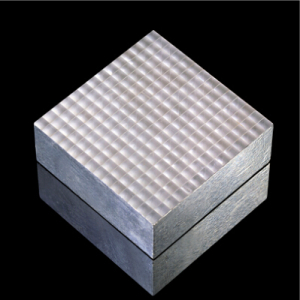
\includegraphics[scale=0.5]{img/LysoSegmented.png}
	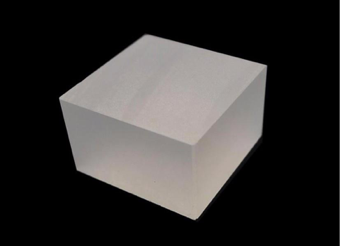
\includegraphics[scale=0.6]{img/LysoMono.png}
	\caption{\label{fig.lyso} LYSO crystals. Left: segmented; right: monolithic.  }
\end{figure}

Most of today's top-of-the-line PET scanners are based in  Lutetium oxyorthosilicate (LSO) or  
Lutetium Ytrium oxyorthosilicate (LYSO) crystals, readout by light sensitive detectors (the field is swiftly replacing photomultipliers by  SiPMs). The crystals, in turn, can be segmented (figure \ref{fig.lyso}--left), forming a matrix
of small pixels (typically $3\times 3 \times 24 \mathrm{mm^3}$), where each pixel is readout by one SIPM, or monolithic (figure \ref{fig.lyso}--right), that is, a single block readout by a matrix of SiPMs, which views the whole crystal. LYSO detectors
are characterised by: a) high density ($\rho_{LYSO} =7.4~\mathrm{g/cm^3}$) and small attenuation length 
($\lambda_{LYSO} =12$~mm for gammas of 511 keV), which permits very compact devices; b) large photon yield
($Y_{LYSO} =14000$~photons for a 511 keV gamma) which result in good energy resolution 
$\sigma^E_{LYSO} \sim12-15$~\% FWHM, for 511 keV gammas); a fast decay scintillation decay constant
($\tau_{LYSO} = 40$~ns), which permits good Coincidence Resolving Time (CRT), essential for TOF applications. 

To achieve good spatial resolution LYSO crystals are finely instrumented. For example, a segmented detector of pixel size $3 \times 3 ~\mathrm{mm^2}$~achieves a rms resolution $\sim \mathrm{3 mm/\sqrt{12} = 0.87~ mm}$~(2 mm FWHM). The resolution in the depth of interaction (DOI) of segmented detectors, on the other hand, is mediocre. For example, a crystal of 20 mm thickness, achieves a DOI resolution of  
$\sim \mathrm{20 mm/\sqrt{12} = 5.8~ mm}$~rms or about 13 mm FWHM. Monolithic detectors used the pattern information recorded by the SiPM matrix to infer the three spatial coordinates, improving the DOI resolution to some 5 mm. 

\subsubsection*{Sources of noise in a PET scanner and TOF measurements}

The reconstruction of the image in a PET system requires crossing many LORs which in turn define one emission point in the area under study. A LOR can be formed by: 1) a {\bf true coincidence}, which occur when both photons from an annihilation event are detected, neither photon undergoes any form of interaction prior to detection, and no other event is detected within the coincidence time-window; 2)
a {\bf scattered coincidence}, which occurs when one or both detected photons undergo at least one Compton scattering interaction prior to detection;
%Since the direction of the photon changes due to the scattering process, the resulting coincidence event will, most likely, produce a wrong LOR. Scattered coincidences add a background to the true coincidence distribution, decreasing contrast and causing the isotope concentrations to be overestimated. They also add statistical noise to the signal; 
3)  a {\bf random coincidence}, which occurs when two photons, not arising from the same annihilation event, impinge the detectors within the coincidence time window of the system. Both scattered and random coincidences  add statistical noise to the data. 

\paragraph{Photon detection sensitivity}

The sensitivity, $S$~ of a PET scanner represents the relationship between the recorded true coincidences and the true activity of a positron-emitting source. The two principal elements influencing the sensitivity are the scintillation crystal’s efficiency and scanner geometry. The efficiency of the scintillator material is mainly dependent on its density, atomic number, and thickness, whereas the most important geometric component of scanner is the active detection area. For a point source located in the center of a cylindrical scanner of diameter $D$~and axial length $L$, the sensitivity 
can be simply expressed as:
%
\begin{equation}
S = \frac{L}{D} \cdot \epsilon^2 \cdot \xi
\label{eq.sensi}
\end{equation}
%
where $\epsilon$~is the individual crystal (or detection cell) efficiency, and $\xi$~ measures the absorption of the gammas in the crystal (cell), $\xi = e^{-\mu \cdot t}$, where $\mu$~is the linear attenuation coefficient of 511 keV photons in the detector material and $t$~is the crystal (cell) thickness. Note that the factor $\epsilon^2$~comes from the need to form a coincidence with two crystals (cells) with efficiency $\epsilon$.  

Notice that $S$~depends linearly of the axial length ($L$) and absorption ($\xi$) but quadratically of the efficiency, due to the need to form a coincidence with two crystals (cells) with efficiency $\epsilon$. 

\subsubsection*{TOF PET}

\begin{figure}[!htb]
	\centering
	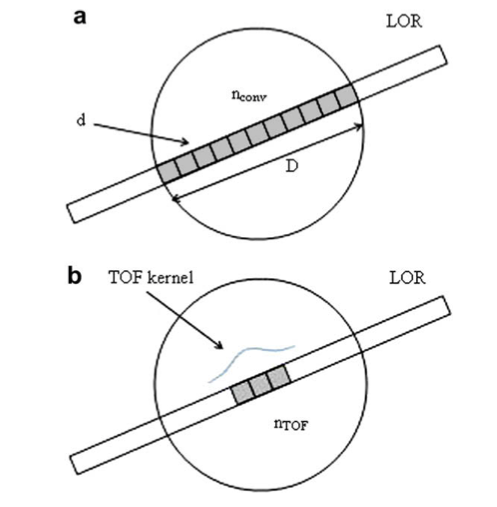
\includegraphics[scale=0.8]{img/TOF.png}
	\caption{\label{fig.tof} (a) In conventional PET reconstruction, all volume elements $n$~ found in the object along the line of response contribute to the noise in each image element, and $n_{conv} = D/d$. (b) In PET--TOF reconstruction, because of the better localisation of each event along the LOR, only the volume elements $n$~ adjacent to the position identified by the measured TOF contribute to the local noise, and $n_{TOF} = \Delta x/d$. The time resolution  $\Delta t$ limits the number of elements contributing to the noise, since it determines the localisation uncertainty $\Delta x$. }
\end{figure}


Time-of-flight (TOF) information is {\em always} used in a PET scanner to determine if two detected photons are in ``time coincidence'' and therefore belong to the same positron annihilation event.
Each detected photon is tagged with a detector position and detection time: if the detection time difference between two photons is smaller than a pre-set coincidence window (typically of the order of a few ns), the two events are considered physically correlated to the same annihilation event. 

Conventional PET reconstruction uses the TOF information only to identify the line along which the annihilation occurred. It is unable, though, to determine which voxel along the line is the source of the two photons; therefore all the voxels along the line are given the same probability of emission (figure \ref{fig.tof}--a). PET--TOF uses the time-of-flight difference to better locate the annihilation position of the emitted positron. The time-of-flight  difference $\Delta t$~ is directly related to the distance $x$~ of the annihilation point from the center of the field of view (FOV), $x = c \Delta t/2$, along the LOR identified by the two detectors in coincidence. The limiting factor to localise the annihilation point is the uncertainty in the measured time difference $\delta \Delta t$, or CRT (Coincidence Resolving Time) of the system. The time resolution is used in the reconstruction algorithm as a kernel for a localisation probability function, as shown in figure \ref{fig.tof}--b. It can be shown that TOF reconstruction is equivalent to an amplification of the PET scanner sensitivity, according to:
%
\begin{equation}
S_{tof} = \frac{D}{\delta x} S_{conv}
\label{eq.sensiTOF}
\end{equation}
%
where $S_{tof}$~is the sensitivity of a PET-TOF system, $S_{conv}$~is the sensitivity of a conventional scanner, 
$D$~is the diameter of the object being imaged and $\delta x = c \delta \Delta t/2 \propto CRT$, 
thus, $S_{tof} \propto \frac{D}{CRT} S_{conv}$. It follows that the gain in sensitivity is directly proportional to the size of the patient and inversely proportional to the CRT. In other words, large patients will particularly benefit from TOF reconstruction.

Currently there is a commercial system based in LYSO crystals, the GEMINI of Philips\footcite{GEMINI}, capable to reach a CRT of 600 ps. Laboratory setups with LYSO crystals reach values in the range of 150--300 ps, depending on the experimental conditions. For example Ferri et al\footcite{LysoFBK}
 report measurements using a pair of small LYSO crystals 
($3 \times 3 \times 5 {\rm mm^3}$) readout by high-fill factor SiPMs. With this setup, a CRT of $157\pm 5$~ ps was found at ambient temperature.

\subsubsection*{Physical properties of liquid xenon relevant for PET}

Xenon is a noble gas. It responds to the interaction of ionizing radiation producing about 60 photons per keV of deposited energy. The emitted photons have wavelengths in the ultraviolet range (VUV)
with an average wavelength of 178 nm. The scintillation signal is fast 
(see below) and can thus result in an excellent CRT.  In its liquid phase (at a temperature of $\sim$ 160 K and atmospheric pressure) LXe has a reasonable high density (3 g/cm$^3$) and an acceptable attenuation length (36 mm), which makes it suitable for PET applications. Its main attractive features are:

\begin{enumerate}
\item {\bf A high scintillation yield (30,000 photons per 511 keV gamma)}, twice as large as that of LYSO. 
\item {\bf LXe is a continuous medium with uniform response}. The design of a compact system is much simpler, then, than when using solid detectors of fixed shape. It is also possible to provide a 3D measurement of the interaction point, and, thus, a high resolution measurement of the DOI. Furthermore, in LXe it is possible to identify Compton events depositing all its energy in the detector as separate-site interaction, due to its relatively large interaction length. This increases the sensitivity of the system, since those events can, in principle, be used for image reconstruction. 
\item {\bf The temperature of LXe at atmospheric pressure (160 K or -113 C)} is hot enough as to permit a simple cryostat, as well as normal operation of the SiPMs, but cold enough to reduce the dark current rate (DCR) of the SiPMs by a factor $\sim 2^{13}$, thus making it essentially negligible. 
\item {\bf The cost of LXe is 3 \euro/cc} to be compared with $\sim$ 40-50 \euro/cc in the case of LYSO. 
 \end{enumerate}

%The first idea of using a LXe time projection chamber for PET was proposed in 1993 by Chepel \cite{chepelFirst}. 
The possibility of building a LXe PET based on the excellent properties of LXe as scintillator was first suggested by Lavoie in 1976  \footcite{lavoie}, and the study of this type of PET was carried out by the Waseda group \footcite{Doke1,Nishikido2,Nishikido1}. 

\subsubsection*{PETALO}


\begin{figure}[!htbp]
	\centering
	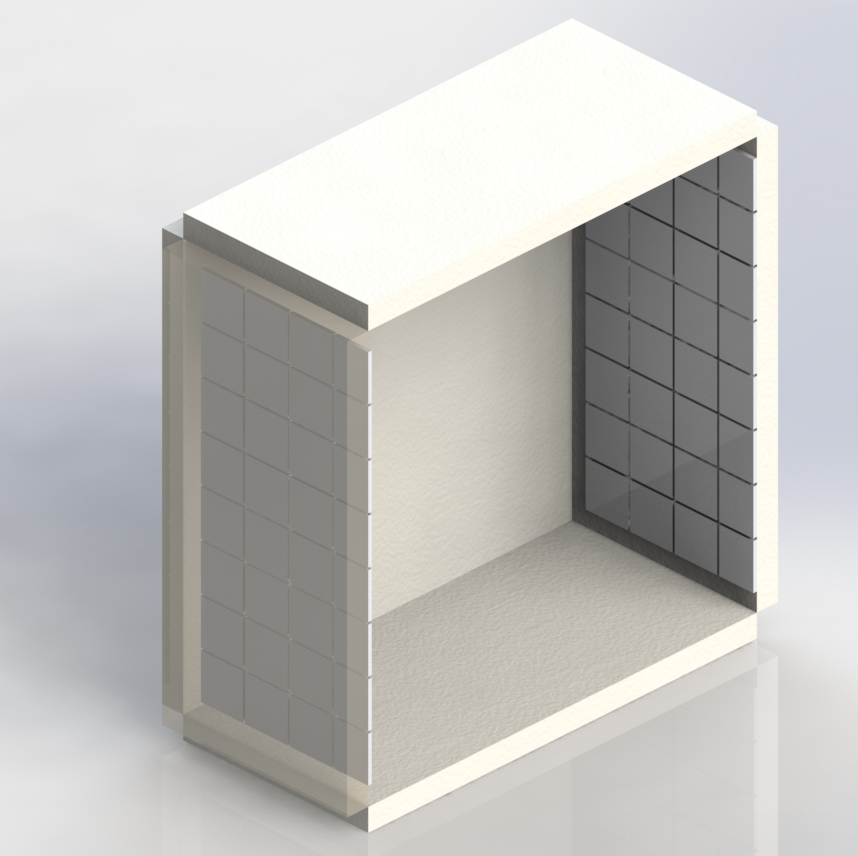
\includegraphics[scale=0.20]{img/Box_2faces_1.jpg}
	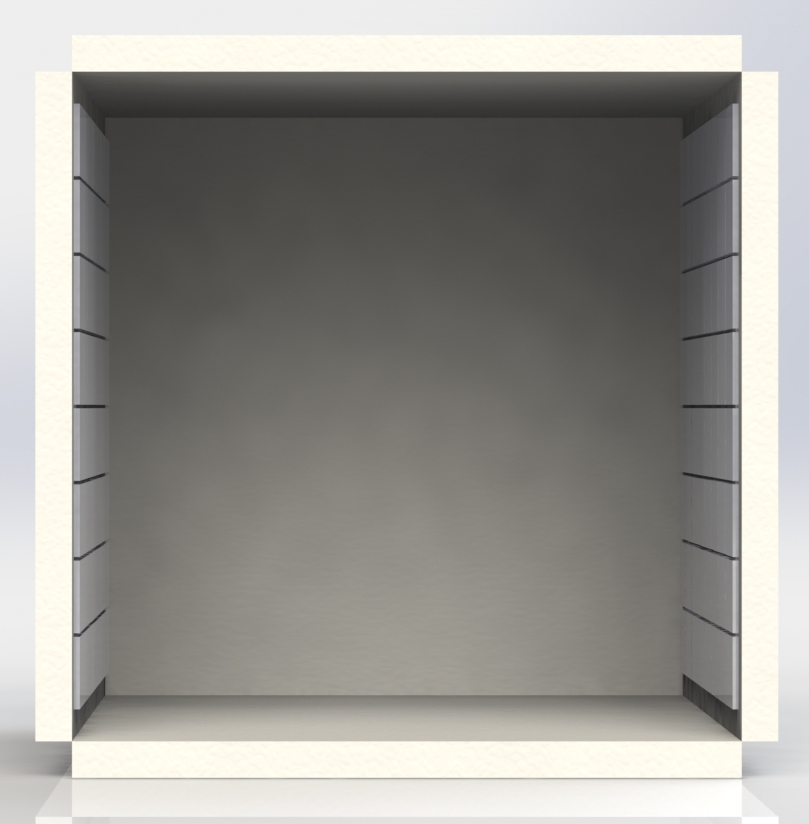
\includegraphics[scale=0.20]{img/Box_2faces_3.jpg}
	\caption{The LXSC2 instruments the entry and exit faces of the box (relative to the photon line of flight) with silicon photomultipliers (SiPMs), which can be eventually coated with TPB. The non-instrumented faces are covered by reflecting Teflon (optionally also coated with TPB).}\label{fig.box} 
\end{figure}
%\begin{figure}[!htbp]
%	\centering
%	\includegraphics[scale=0.6]{../img/LXSC2.pdf}
%	\caption{The LXSC2 instruments the entry and exit faces of the box (relative to the photon line of flight) with silicon photomultipliers (SiPMs), which can be eventually coated with TPB. The non-instrumented faces are covered by reflecting Teflon (optionally also coated with TPB).}\label{fig.box} 
%\end{figure}

PETALO (Positron Electron TOF Apparatus using Liquid xenOn) is a proposed new type of PET scanner which exploits the copious scintillation of liquid xenon and the availability of state-of-the-art SiPMs and fast electronics designed to maximise TOF performance \footcite{Petalo2015}. The detector building block is the liquid xenon scintillating cell (LXSC). The cell shape and dimensions can be optimised depending on the intended application. In particular, the LXSC2 instruments the entry and exit faces of the box (relative to the gammas line of flight) with silicon photomultipliers, while all the other faces are covered with a reflecting material such as Teflon. The SiPMs are read out by ASICs optimised for excellent timing resolution. 
 %PETALO is a compact, homogenous and highly efficient detector which shares many of the desirable properties of monolithic crystals, with the added advantage of high yield and fast scintillation offered by liquid xenon, low noise due to cryogenic operations which virtually eliminates the SiPMs DCR, and the potential of low cost. 
%

The energy resolution and spatial resolution of the LXSC2 instrumented with 6 mm SiPMs has been studied
by Gomez-Cadenas et al.\footcite{Petalo2015}. The energy resolution was found to be 12\% FWHM for 511 keV gammas. The spatial resolution in the three coordinates was found to be 2 mm FWHM. Both the energy resolution and the spatial resolution in the (x,y) coordinates (transverse to the gammas line of flight) were of the same order than that obtained by top of the line LYSO scanners. The resolution in the longitudinal coordinate, measuring the depth of interaction (DOI) was obtained by computing the ratio between the
total signal recorded in the instrumented entry and exit face. A DOI resolution of 2 mm is much better than that obtained by segmented LYSO crystals (unless the thickness of the crystal is very small), and compares with the best results obtained using monolithic crystals \footcite{VanDamm2011}.
%
\subsection*{VUV-sensitive SiPMs versus SiPMs coated with TPB}
%
%\begin{figure}[!htbp]
%	\centering
%	\includegraphics[scale=0.6]{../img/PDEVUV.png}
%	\caption{Photo detection efficiency (PDE) of different VUV sensitive SiPMs
%	(from http://neutrino.physics.ucdavis.edu/indico/contribAuthorDisplay.py?contribId=61\&authorId=0\&sessionId=2\&confId=17). The MEG devices are
%	manufactured by Hamamatsu Photonics, while the FBK-2010 and the RGB-HD
%	are manufactured by FBK.  }\label{fig.vuv} 
%\end{figure}
%
%\begin{figure}[!htbp]
%	\centering
%	\includegraphics[scale=0.6]{../img/TPBEfficiency.png}
%	\caption{Visible re-emission spectrum for a TPB film illuminated with 
%	128, 160, 175, and 250 nm light. All spectra are normalized to unit area.
%	(from \cite{Gehman:2011xm}).  }\label{fig.tpb} 
%\end{figure}
%
%\begin{figure}[!htbp]
%	\centering
%	\includegraphics[scale=0.6]{../img/TPBSpectrum.png}
%	\caption{Total integrated fluorescence efficiency for a thin layer of TPB, as a function of input  photon wavelength
%	(from \cite{Gehman:2011xm}).  }\label{fig.tpbeff} 
%\end{figure}
%
%\begin{figure}[!htbp]
%	\centering
%	\includegraphics[scale=0.6]{../img/PetaloTOF/TpBDecayConstant.png}
%	\caption{Evolution of the decay constant of TPB as a function of the thickness of the TPB layer compared
%	with the thickness of the substrate (a thin quartz film). The TPB decay constant decreases as the thickness of the TPB layer (thus its concentration) increases, reaching an asymptotic value of 2.2 ns.   
%	(from \cite{TPBtau}).  }\label{fig.tpbtau} 
%\end{figure}
%

The scintillation light of LXe peaks around 178 nm (VUV region). Therefore the LXSC2 needs to be instrumented either with VUV-sensitive SiPMs (as for example the upgraded LXe calorimeter of the 
MEG experiment \footcite{Ogawa:2015ucj}) or by conventional SiPMs coated with a wavelength shifter such as tetraphenyl butadiene (TPB) (as for example in the NEXT experiment \footcite{Alvarez:2013gxa}). 
The VUV-SiPMs tested for the MEG as well as for the future nEXO 
experiment \footcite{Ogawa:2015ucj,Ostrovskiy:2015oja} reach a PDE of about 
15\%. Further improvements of the technology could eventually result in a PDE of 20\% .  Conventional SiPMs can reach today a PDE of around 50\%.When they are coated with a thin layer of TPB, the VUV light is absorbed by the wavelength shifter with an efficiency of 80\% \footcite{Gehman:2011xm}
shifted to $\sim$ 430 nm and re-emitted isotropically. The decay constant of TPB has been measured  in thin films \footcite{TPBtau} and a value of 2.2 ns is found for sufficiently large TPB concentrations. 

\subsubsection*{PETALO as a PET-TOF scanner}
The potential of PETALO as a a PET-TOF scanner has been recently studied by Gomez-Cadenas et al.,  \footcite{PetaloTOF}. The scintillation in xenon is parameterised in terms of two decay constants:

 \begin{figure}[!bhtp]
	\centering
	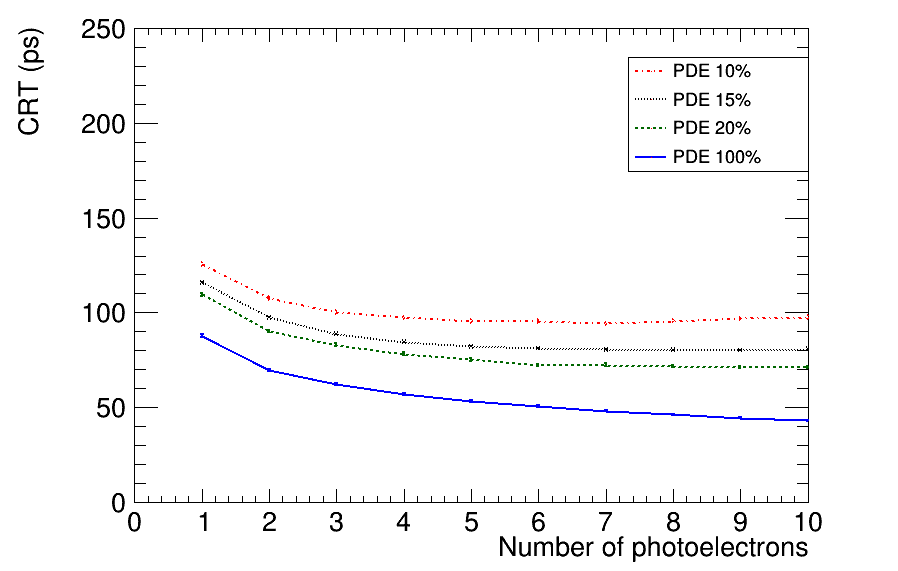
\includegraphics[scale=0.40]{img/lxe_noCher_avg_npe_phys.png}
	\caption{\label{fig.crt_avg_LXe} CRT as a function of the number of photoelectrons used to compute $\Delta t$, for LXe. The CRT is shown for several values of the PDE (from \cite{PetaloTOF}).}
\end{figure}

\begin{equation}
I(t) = N_\gamma (0.07 \times \frac{e^{-t/\tau_1}}{\tau_1} + 0.93 \times \frac{e^{-t/\tau_2}}{\tau_2})
\label{eq.scint}
\end{equation}
where $\tau_1 = 2.2$~ns and $\tau_2 = 27$~ns. Thus, xenon scintillation is not only more copious (by a factor two) but also much faster than scintillation in LYSO. Using VUV-sensitive SiPMs a CRT of 70 ps is found for a PDE of 20 \% (80 ps for a PDE of 15\%, see figure \ref{fig.crt_avg_LXe}). Using conventional SiPMs coated with TPB, the CRT varies between 130 and 155 ps, depending on the (poorly known) value of the TPB decay constant. This results show the
potential of the PETALO concept as a PET-TOF scanner.  

\subsubsection*{Resolving Compton interactions:}

\begin{figure}[!htbp]
	\centering
	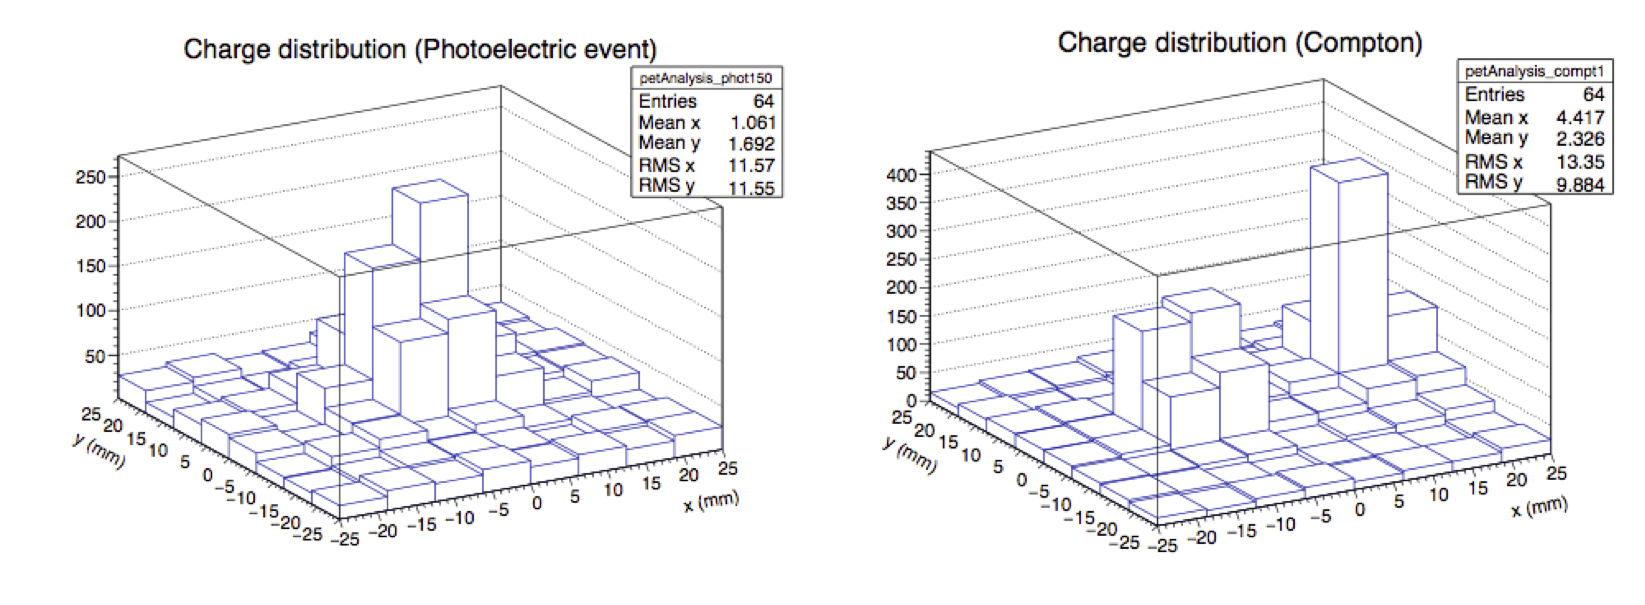
\includegraphics[scale=0.6]{img/Compton.png}
	\caption{The LXSC2 can distinguish well between 1-site photoelectric events (left panel) and
	Compton events, such as the 2-site Compton event shown in the right panel.}\label{fig.Compton} 
\end{figure}

Photoelectric interactions are a relatively small fraction of the total number of interactions in LXe (22\%) as well as in LYSO (33\%). The bulk of Compton interactions can result either in contained (when the scatter gamma produces a cascade that does not escape the detector) or non contained events. Non contained events do not deposit the full energy of the gamma in the detector and can be rejected. However, the large fraction of contained Compton events (60\% for the LXSC and larger for the denser crystals of LYSO) introduce a significant distortion of the position and contribute to the noise and to spoil the CRT. 

An important advantage of the LXSC2 is that multiple-site hits can be identified (the system measures true 3D points). Thus Compton events can either be rejected, or added to the imaging sample, in the case of 2-site interactions where each vertex is clearly identified (an example is shown in figure \ref{fig.Compton}), thus increasing sizeably the efficiency.  
%

\subsubsection*{PETALO as a Full-Body PET}
%
\begin{figure}[!htb]
	\centering
	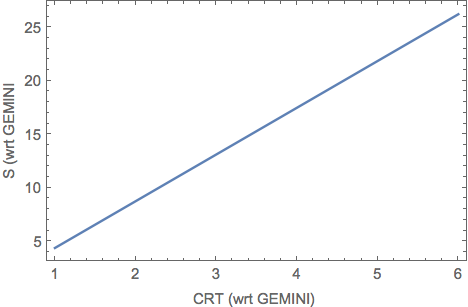
\includegraphics[scale=0.6]{img/RelativeSensitivity.png}
	\caption{\label{fig.rsensi} Relative sensitivity of a PETALO-TOF-FBP scanner w.r.t the the current top-end PET-TOF scanner, the GEMINI of Philips as a function of the relative CTR.  }
\end{figure}


A major application of the PETALO concept would be the construction of a ``Full Body PET'' (FBP), of axial dimensions in the range of 70-100 cm, exploiting the low cost and the excellent performance offered by LXe. In addition to the superb energy resolution and spatial resolution a PETALO--FBP scanner would offer a much increased sensitivity w.r.t. conventional PET devices. To illustrate this point, we combine equations \ref{eq.sensi} and \ref{eq.sensiTOF} to write the relative sensitivity of two PET scanners, $p_1,p_2$~ having the same bore and scanning a patient of the same dimensions as:

\begin{equation}
S(p_1,p_2) = \frac{L_1} {L_2}\frac{CTR_1} {CTR_2}\frac{\epsilon_1} {\epsilon_2}\frac{e^{-\mu_1 t_1}} {e^{-\mu_2 t_2}}
\label{eq.srel}
\end{equation}
%
where $L_i,CTR_i,\epsilon_1,\mu_i,t_i, i=1,2$~are the axial length, CTR, detector efficiency, linear attenuation coefficient and crystal (cell) thickness for scanners $p_1,p_2$.

We can now use equation \ref{eq.srel} to compare the performance of a 1 m axial length PETALO-TOF-FBP scanner using LXe ($\mu = 36$~mm) and based in LXSC2 cells of 50 mm thickness with the current top-end PET-TOF scanner, the GEMINI of Philips, using LYSO crystals ($\mu = 12$~mm) of 25 mm thickness. Figure \ref{fig.rsensi} shows the improvement in sensitivity as a function of the improvement in CTR, assuming that the detection efficiency of both systems is the same. A factor 10 improvement is obtained if the PETALO scanner achieves an overall CTR of 240 ps, and a factor 20 for a CTR of 130 ps, which is feasible even using cost-competitive SiPMs coated with TPB. 

The assumption that a LYSO crystal and an LXSC cell can have similar efficiencies is important and deserves some discussion. The factors that affect the efficiency are: i) the photoelectric fraction; ii) the fraction of Compton events that can be used for imaging; iii) the energy window to accept events; iv) the time window to accept events; the packing factor of the crystals (e.g, the amount of dead space between crystals needed for packing). Of this list, LYSO has a better photoelectric fraction than LXE (0.33 versus 0.2); Compton events can be better distinguished in LXe than in LYSO, allowing to increase the fraction of events useful for imaging in the LXSC2; the energy window of both system is similar, (energy resolution is of the same order); the time window in LXe is better than in LYSO (scintillation is faster); the packing in LXe is better than in LYSO, since LXe is a continuous medium and the LXSC cells can be tailored to minimise dead areas. Thus, the LXSC offers better Compton identification, time window and compactness to compensate the lower photoelectric fraction. 
%



\subsection*{Objetivos generales y adecuación al Programa Estatal de I+D+i orientada a los Retos de la Sociedad / General objectives and match to the National Programme for research aimed at the Challenges of Society}

\subsubsection*{Overall objectives}
The overall objectives of this research proposal are: a) an exhaustive investigation of the physics of scintillation in liquid xenon and its potential for medical imaging. Specifically, we propose:
\begin{enumerate}
\item A precise measurement of the yield of 511 keV photons and its time dependence, two crucial parameters for PET performance which are still today affected of considerable systematic uncertainties.
\item A systematic measurement of the performance of the LXSC (including energy resolution, spatial resolution and CRT). Two configurations will be studied, one with two planes of SiPMs per cell (LXSC2) and another with a single plane (LXSC1), in order to assess quantitatively the tradeoff between cost and performance.
\item A systematic measurement of the performance of different SiPM in LXe. We will study the dependence of the time resolution with the SiPM capacitance, the reduction of dark current, and measure the CRT that can be achieved with VUV--sensitive SiPMs and with SiPMs coated with TPB. 
\item A systematic evaluation of state-of-the-art custom ASIC electronics for TOF-PET. Specifically we will study the performance of the TOF PET ASIC from PETSYS \footnote{http://www.petsyselectronics.com/web/public/products/1}. 
\item We also intent to collaborate with a group of researchers from UB \footnote{Gascon, Graciani, Garrido} to evaluate other alternatives, such as FlexToT \footcite{Trenado:2014vba}. 
\item We will study the eventual operation of PETSYS and/or FlexToT electronics in LXe cryogenic conditions.
\item In collaboration with the UB group, we will study the performance of fast detectors (such as MCPs or SPADs) with fast custom electronics (provided by the UB group) with the aim of detecting and exploiting for CRT measurements the Cherenkov light produced in xenon.  
\item Last but not least, we propose the construction, commissioning and operation of a prototype of PETALO, which we call PEP (Petalo Prototype). PEP will be built in three stages. Stage 1 (P1) will operate a LXSC in a small cryostat. The gas system and the common cryogenic elements will be developed, and studies of yield, timing, energy and spatial resolution will be carried out, as well as studied to characterise SiPMs and electronics.  Stage 2 (P2), will add a second LXSC for detailed CTR measurements. Finally, we will build the full PEP demonstrator equipped with 15 LXSC. 
\end{enumerate}

The objectives presented in this project are very well aligned to the Spanish program for science. They involve a direct technology transfer from basic science in particle physics to a medical imaging application of high social impact (Reto 1: Salud). It involves a multidisciplinary collaboration between physicist, engineers and medical doctors. And it has a large potential for generating commercial spinoffs, including the possibility of a break through in  PET-TOF, and PET-FBP technology.  


\subsection*{Objetivos específicos / Specific objectives}
%

\input{src/ObjDet.tex}
\input{src/ObjAsic.tex}
\input{src/ObjImg.tex}

\subsection*{Metodolog\'ia / Methodology}

%4. El detalle de la metodologia propuesta en cada uno de los subproyectos participantes

\subsubsection*{Methodology of the DET subproject}

\subsubsection*{P2}

\begin{figure}[!htb]
	\centering
	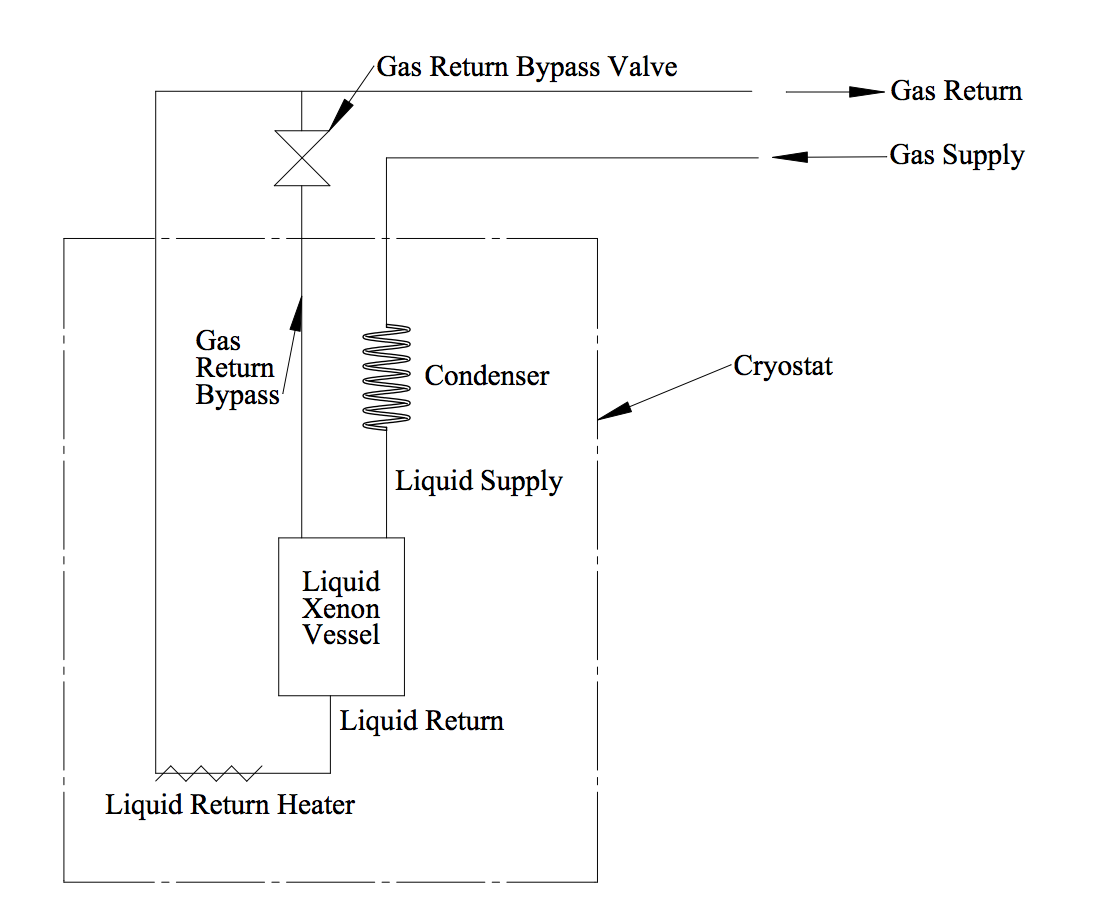
\includegraphics[scale=0.45]{img/CryoGas1.png}
	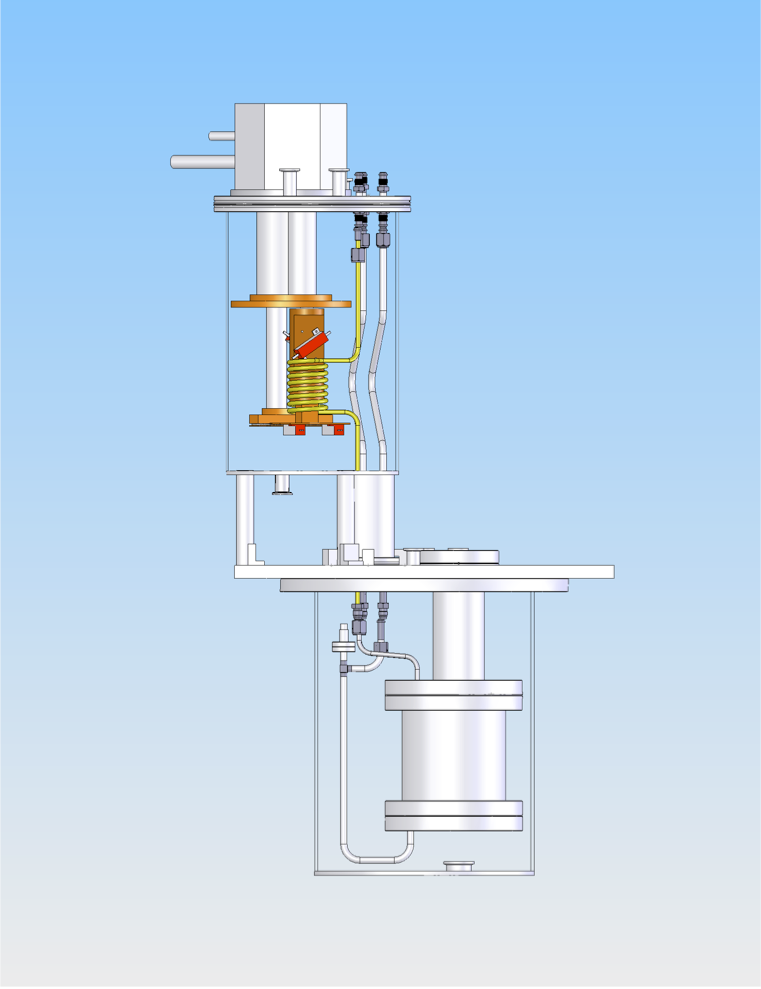
\includegraphics[scale=0.45]{img/CryoGas2.png}
	\caption{\label{fig.cryo} Left: P2 components. Right: a drawing of P2. The upper part of the cryostat holds the condenser, and the lower part holds the liquid xenon vessel (LXV). The P2 experiments will be carried out placing several setups inside the LXV.}
\end{figure}

\begin{figure}[!htb]
	\centering
	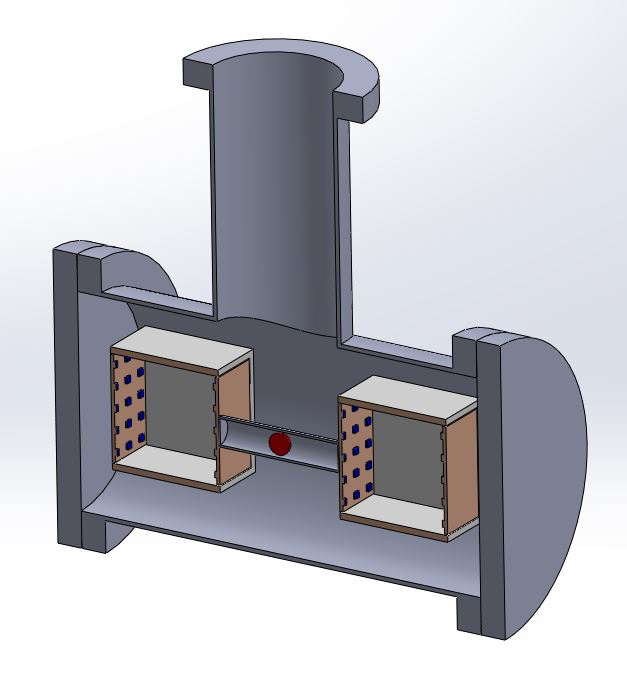
\includegraphics[scale=0.45]{img/P2.png}
	\caption{\label{fig.P2} A drawing showing the experimental arrangement in P2. The setup shows two LXSC2 with the radioactive source in a sealed container. }
\end{figure}

Figure \ref{fig.cryo}--left shows the components of the P2 setup. Room temperature gas flows to the condenser. Liquid drips into the vessel, and cool gas returns through the gas return line. The gas can also return through the liquid return line when no liquid is present. Figure \ref{fig.cryo}--right shows a drawing of P2. The upper part of the cryostat holds the condenser, and the lower part holds the liquid xenon vessel (LXV). The P2 experiments will be carried out placing several setups inside the LXV (figure \ref{fig.P2}). 

The construction of the P2 prototype involves three well defined tasks: 
\begin{enumerate}
\item {\bf Construction of the cooling system}, which includes the cryocooler, the condenser, the LXe vessel and the cryostats.  The system includes a vacuum pump to make vacuum in the LXe vessel before the liquid fill.
\item {\bf Construction of the gas system}, which includes the piping, recirculation pump and getter. The system includes an RGA to monitor the levels of impurities in the system. 
\item {\bf Construction of the experimental setups}. Two LXSC2 model A, and two LXSC2 model B will be 
manufactured:
\begin{itemize}
\item {\em Model A}, will be LXSC2 of $50 \times 50 \times 50 \mathrm{~mm^3}$, with two instrumented faces and all the others covered by reflective Teflon. Each instrumented face will deploy a matrix of $8 \times 8$~SiPMs of 6 mm length called Dice Board (DB). The SiPMs will be of conventional type, coated with TPB.
\item {\em Model B}, will be boxes of $25 \times 25 \times 50 \mathrm{~mm^3}$, with two instrumented faces and all the others covered by reflective Teflon. Each instrumented face will deploy a DB of $8 \times 8$~SiPMs of 3 mm length. The SiPMs will be VUV-sensitive (currently the maximum size of VUV sensitive SiPMs is 3 mm). 
\end{itemize}
\end{enumerate}

The three tasks can be carried out essentially in parallel, since most of the parts required are manufactured by industrial suppliers and can be ordered at the same time. The estimated time for the construction of P2 is 12 months. 

%A full-time mechanical engineer with expertise in cryogenics is needed for the design, assembly and commissioning of the system. The engineer will have the support of the IFIC engineering group and the support of the NEXT experiment, in particular concerning the construction and commissioning of the gas system (which will be a simplified version of the gas system built for the NEXT-DEMO detector, currently operating at IFIC). The estimated time needed to design, construct and commission P2 is one year. 

%Specifically, we will build two LXSC2 equipped with VUV-sensitive SiPMs (LXSC2-VUV) and two LXSC2 equipped with conventional SiPMs coated with TPB (LXSC2-TPB). The dimensions of the 
%\begin{enumerate}
%\item {\bf Yield}: the measurement of scintillation yield and time dependence in LXe will be done with a LXSC2 of 
%$25 \times 25 \times 25 \mathrm{~mm^3}$~equipped with 3 mm VUV-sensitive SiPMs. (LXSC2-VUV-1).
%\item {\bf Resolution}: 
 
%The first round of measurements can be done with a single LXSC, while the second round of measurements will be done with two LXSCs facing each other. A sealed tube (called the radioactive source holder, RSH), kept at a light vacuum will be placed in the middle of the two LXSC and will hold the radioactive Na-22 source for coincidence studies. The gammas within the angular acceptance of the RSH will exit the tube and enter the LXSCs through thin mylar windows. Gammas outside the acceptance will be attenuated by the LXe filling the vessel (and the LXSCs). 


\subsubsection*{Simulation and reconstruction}
While the P2 detector is being built, a full simulation (called SIMPLE) of P2, PEP and a future full-body PETALO scanner will be developed. The simulation is essential to understand the response of the prototypes, as well as to prepare and test the imaging algorithms.

In parallel to SIMPLE a reconstruction and analysis framework (RAP) will be written. RAP will be tested on Monte Carlo data, so that it is available when P2 starts operation. 

%Based on SIMPLE and RAP, algorithms for imaging (calculation of LORs, filtered backprojection , TOF algorithms, maximum Likelihood expectation methods and machine learning methods) will be prepared. 

SIMPLE and RAP will be developed in parallel with P2 construction (12 months).  

\subsubsection*{Operation of the P2 prototype}
The operation of P2 will address objectives 1-4 of the project. P2 will be operated during a period of 12 months, in parallel with the construction of PEP. The operation of P2 will be coordinated by the DET subproject, but personnel from the other two subprojects as well as from the UB group will participate in the experiments and data analysis. 

%permit a number of measurements, essential to understand the performance of LXe and its potential for medical imaging. Specifically, P2 will provide:
%\begin{enumerate}
%\item A precise measurement of the yield of 511 keV photons and its time dependence, two crucial parameters for PET performance which are still today affected of considerable systematic uncertainties.
%\item A systematic measurement of the performance of the LXSC (including energy resolution, spatial resolution and CRT). 
%\item A systematic measurement of the performance of different SiPM in LXe. We will study the dependence of the time resolution with the SiPM capacitance, the reduction of dark current, and measure the CRT that can be achieved with VUV--sensitive SiPMs and with SiPMs coated with TPB. 
%\item A systematic evaluation of state-of-the-art custom ASIC electronics for TOF-PET. Specifically we will study the performance of the TOF PET ASIC from PETSYS \footnote{http://www.petsyselectronics.com/web/public/products/1}. 
%\item We also intent to collaborate with a group of researchers from UB \footnote{PI D. Gasc\'on, henceforth UBG} to evaluate other alternatives, such as FlexToT \footcite{Trenado:2014vba}. 
%\item We will study the eventual operation of PETSYS and/or FlexToT electronics in LXe cryogenic conditions.
%\item In collaboration with the UBG, we will study the performance of fast detectors (such as MCPs or SPADs) with fast custom electronics (provided by the UBG) with the aim of detecting and exploiting for CRT measurements the Cherenkov light produced in xenon.  
%\end{enumerate}
%
%The operation of P2 and the analysis of the P2 data will extend over 18 months, in parallel with the construction of the larger PEP prototype. The operation of P2 requires from the DET subproject a post-doc fully dedicated to perform the experiments needed to study the various parameters and analyse the data. This project is also ideal for a graduate student. The post-doc and the student will work under the direct supervision of the PI. The operation and analysis of P2 data will also benefit from the collaboration of the ASIC subgroup and the UBG (items 4 to 6).

\subsubsection*{Construction and initial commissioning of the PEP prototype}

\begin{figure}[!htb]
	\centering
	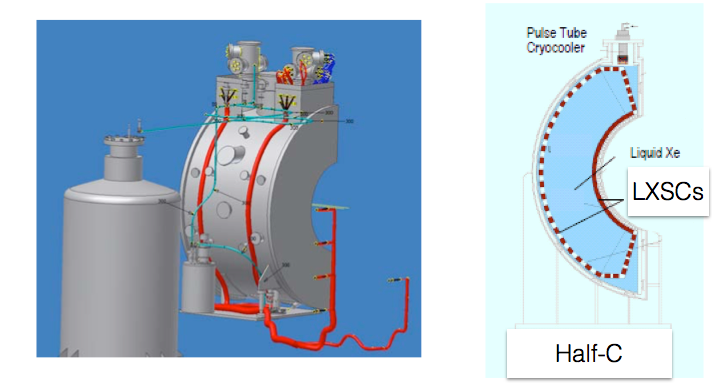
\includegraphics[scale=0.45]{img/HalfC.png}
	\caption{\label{fig.halfC} The half-C cryostat concept pioneer by the MEG experiment can be applied directly
	to PEP and a future large-scale PETALO scanner. }
\end{figure}

Figure \ref{fig.halfC} shows the half-C cryostat concept pioneer by the MEG experiment, which can be applied directly to PEP and a future large-scale PETALO scanner. The detector combines two half-C's in which the entry
faces are thin steel sheets (about 0.4 mm thick), while the rest of the container is reinforced to hold comfortably
	the pressure difference in the vacuum interfaces.  The cryocooler is directly coupled to the cryostat.    

The two half-C's of PEP will close to form a ring of inner diameter 230 mm, which will host 14-LXSCs
of dimensions  $50 \times 50 \time 25\mathrm{~mm^3}$~read out by a single matrix of $8 \times 8$~6-mm blue sensitive SiPMs coated with TPB. PEP implements one layer of SiPMs (rather than two) to reduce costs. The thickness of the LXe cell is reduced accordingly to half of the nominal thickness of the LXSC2. 

The construction of PEP will take 12 months. The DET subproject will be in charge of the cryogenics, gas system and mechanics of the LXSC assembly, while the ASIC subproject will be in charge of the instrumentation and electronics of the LXSCs. 

%The construction of PEP requires a full-time engineer for 18 months.  


\subsubsection*{Operation of PEP}
PEP will be operated for a period of 6 months at IFIC and will be installed at the hospital LaFe during the last 6 months. The DET group has the responsibility to guarantee correct operation an maintenance of the apparatus. The IMG group has the responsibility of integrating PEP in a clinical environment. 

The initial operation of PEP will allow to measure the technical parameters of the scanner (resolution, sensitivity, CRT, etc.). Operation at the hospital LaFe will focus in the reconstruction of images and the extraction of biomarkers. 

%The post-doc assigned to software in the DET group, as well as the graduate student will participate in the imaging studies that will be led by the IMG group once the detector is fully operational. 

 
\subsubsection*{Methodology of the ASIC subproject.}

\subsubsection*{Electronics and DAQ: the PETSYS solution}
%
\begin{figure}[!htb]
	\centering
	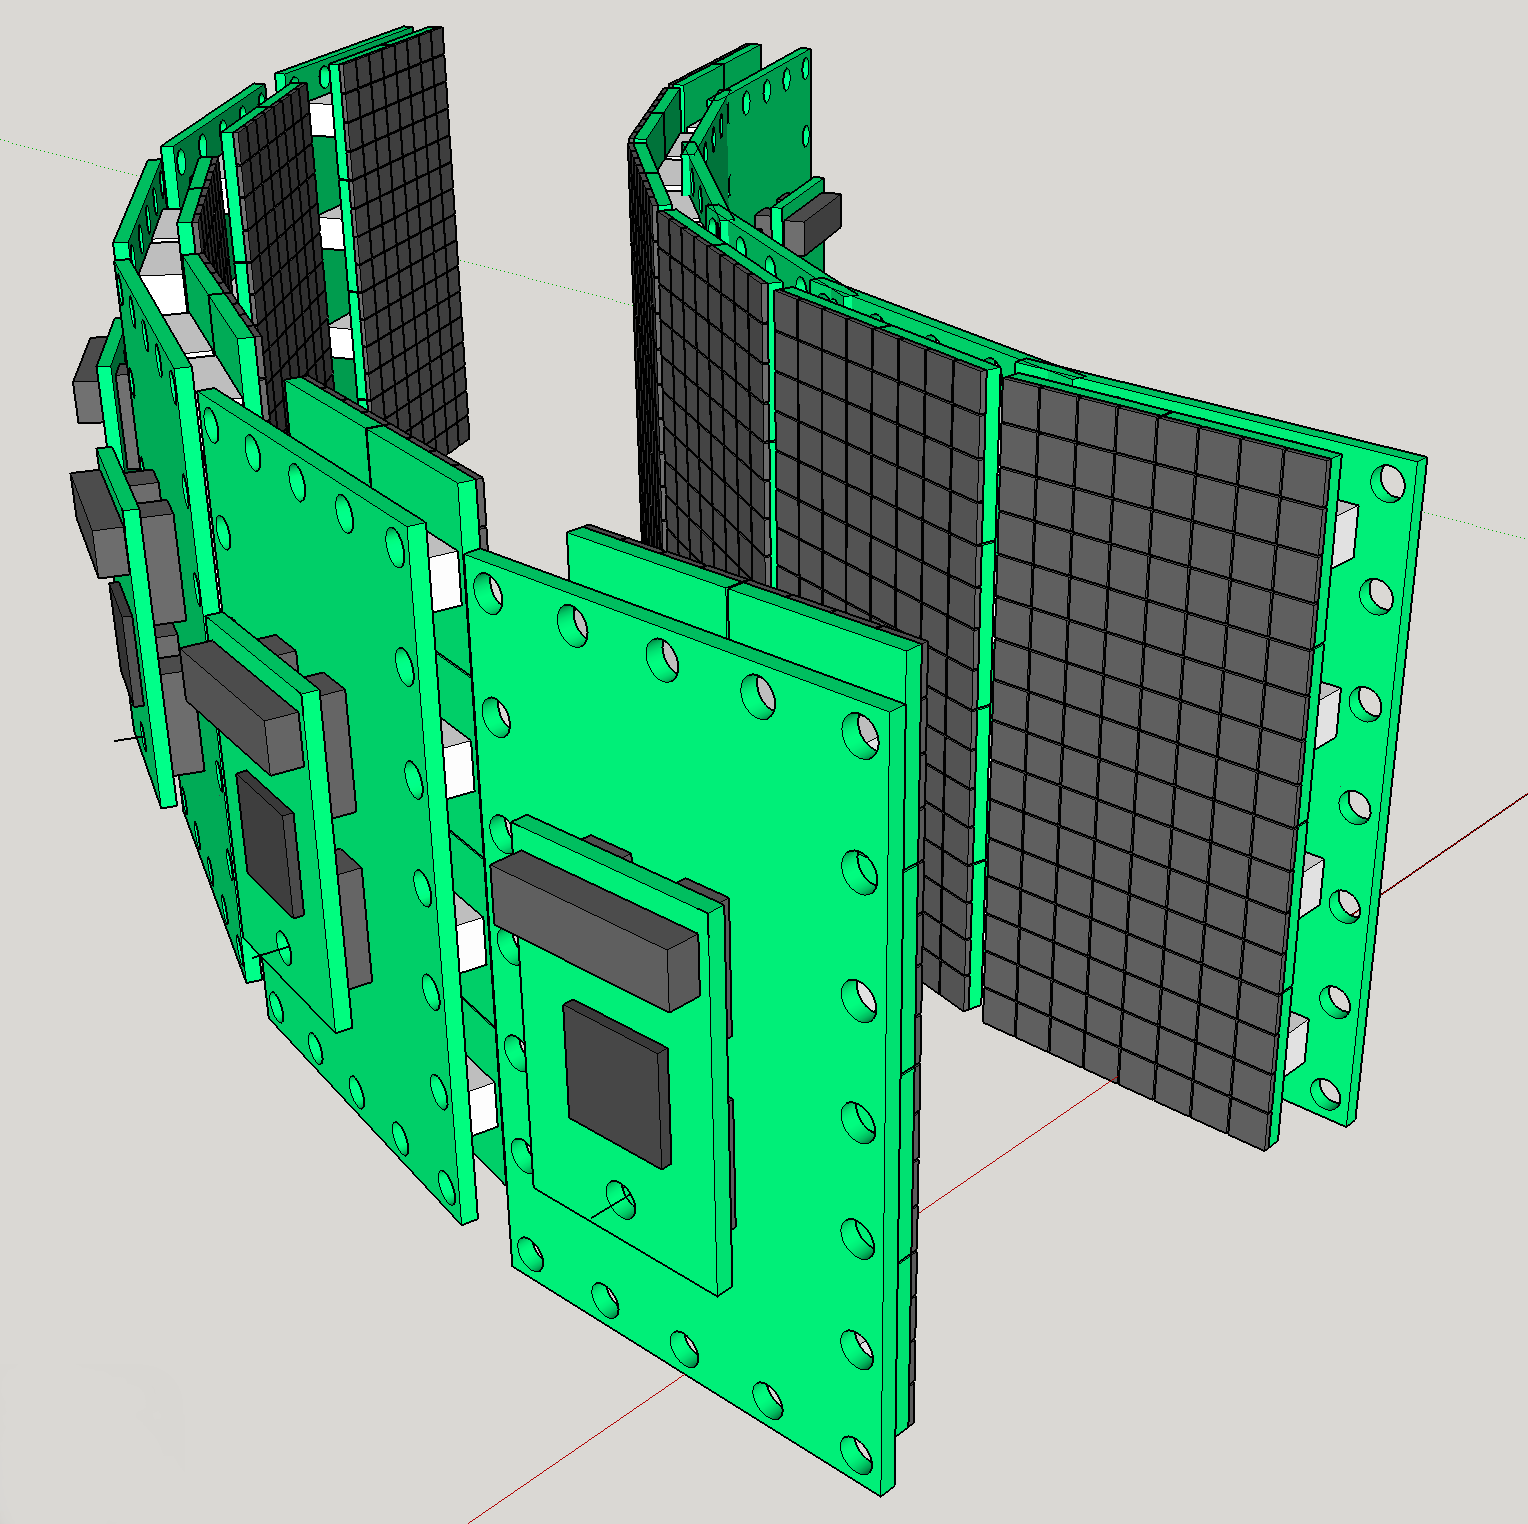
\includegraphics[scale=0.25]{img/PEP.png}
	\caption{\label{fig.pep} A drawing illustrating the arrangement of SiPMs and readout electronics in PEP. }
	\end{figure}

The baseline solution adopted for PETALO is the use of the PETsys TOFPET2 ASIC
\footnote{http://www.petsyselectronics.com/web/website/docs/products/product1/Flyer\%20ASIC\%20TOFPETv2.pdf}, a low power, low noise SiPM readout ASIC
optimised for  time measurement. The ASIC provides signal amplification and discrimination for 64 independent channels. It uses a low threshold
for  timing and a high threshold for accepting the event. Both thresholds are separately configurable for each channel. When any of the 64 channels exceeds the high threshold the ASIC fires, providing a record giving the channel number, the time and the amplitude of the event. The ASIC has large dynamic range (1500 pC) and can handle large
capacitance (thus large SiPMs), offering a SNR of 25 dB for an
input capacitance of 320pF. A fine TDC binning (25 ps) makes it suitable for CRT measurements in the range
of 100 ps. Each channel can handle a hit rate of 600 kHz, the operation frequency is 200 MHz and the max output
rate is 3.2 Gb/s. The output is fully digital and the power consumption around 10 mW/channel.

The crucial features of the ASIC are its low time resolution (25 ps) and the low amplifier noise (25 ps for 1 photoelectron signal).

PETSYS provides a front-end board (FEBA/A) carrying two ASICs, and therefore capable to handle 128 channels. The board dimensions are very compact $52 \times 25.4 \mathrm{~mm^2}$~and fully compatible with the transverse dimensions of the PEP LXSCs ($50 \times 50 \mathrm{~mm^2}$). Thus, each FEB/A can handle a LXSC2 with a double
layer (entry and exit faces) of $8 \times 8$~6 mm SiPMs. If the FEB/A board can be adapted to work at LXe temperatures (it has currently been tested to work at $-80\,^{\circ}{\rm C}$), this allows a very compact readout solution,
as sketched in figure \ref{fig.pep}. Alternatively, one can extract the analog signals of each LXSC using feedthroughs, which have been already developed in the context of the NEXT experiment.

PEP will deploy 14 LXSCs, instrumented with a single DB-A per cell. Each FEB/A can readout two DBs and therefore 7 FEB/A are needed for the whole system. The low power of the ASIC (about 130 mW per FEB/A) results in a total power dissipation of less than 1 W for the whole system, which is much less of the typical power of a standard cryocooler (about 30 W).

The FEB/A digital signals are routed to a concentrator board called FEB/D. A single FEB/D can handle up to 8 FEB/A (thus we need only one FEB/D for PEP). In turn, the FEB/D board sends data to a DAQ master board that can handle up to 12 FEB/D master boards (a master FEB/D, in turn, can daisy-chain several slave FEB/D cards). Thus, the advantage of the solution offered by PETSYS is that is fully scalable to a large system. This would permit a quick upgrade of PEP towards a commercial/pre-commercial system as an spinoff of this project.

The ASIC subproject will contribute to P2 and PEP fabricating and testing the needed DBs for both prototypes. ASIC is also in charge of procuring, testing and commissioning the PETSYS FEE electronics and DAQ. In addition, ASIC will develop the slow controls of the cryogenic and gas systems.

\subsubsection*{Developing electronics suitable for LXe temperatures}

The reliable operation of electronic systems below the military temperature range also known as low temperature electronics (LTE) is quite a challenging objective in itself. Although LTE exploits some useful effects at the device level which enhance the performance of some key components \footcite{fast_lte_dram} there are some severe drawbacks related to reliability at the package and printed circuit board (PCB) which must be carefully studied.
LTE physics in general show a good behavior of some key parameters in microelectronic processes which improve MOSFET devices characteristics. For instance the carrier's mobility increases with lower temperatures which turns into lower channel resistance. Moreover the saturation velocity which is of main importance in deep submicron device transconductance, gets increased in LXe temperature range \footcite{sat_velocity}. Also leakage current gets reduced in LTE which can have a serious impact in high precision detectors. However the reduction of channel resistance also bears a dangerous side effect, the probability of hot electron trapping in the gate interphase rises. This could lead to a premature aging of the transistors and a wide deviation in analog amplifier characteristics. 
PEP and even PETALO will have to put up with periodical thermal cycles for maintenance and trimming at the development stage and also at the final clinical operation. The mismatch of thermal expansion coefficients of the materials at different points of the electronic circuitry \footcite{lau2012thermal} creates mechanical stress which turns into an accelerated aging, fatigue and even failure. This may happen in the die-package adhesive or soldering for flip-chip solutions but also in the wirebonding in case a direct PCB-die bonding is employed in the DB modules. The same failure mechanism can be observed at the PCB level were the thermal stress can be even worse due to the bigger dimensions. The research team foresees a DB and FEB/A redesign taking into account the thermal stress constraints if they are to be placed inside the sealed container.

\subsubsection*{Studies of fast detectors and electronics: collaboration with CLUES}

As discussed in this proposal, the fast and copious scintillation in LXe may allow a CRT in the vicinity of 70-80 ps. The contribution to the CRT comes in part from the effect of the decay constants and the LXe refraction index (that would result in about 50 ps using the first photoelectron) and the response of detectors (e.g, the intrinsic jitter of a SiPM, which is of the order of 100 ps rms) and electronics (about 30--50 ps rms). In LXe there one could also attempt to use the rather copious Cherenkov light (about 100-200 photons per event, typically oner order of magnitude more than in solid scintillators) to reduce the intrinsic contribution to the CRT from $\sim$50 ps to  $\sim$10 ps. In any case, both the detection of Cherenkov light and scintillation light would benefit from developing fast detectors and electronics, contributing with at most 10 ps to the CRT.

Current photo detection technology needs to progress in order to exploit the fast scintillation and even faster Cherenkov prompt emission light. Progress is required in three aspects:
\begin{enumerate}
\item The intrinsic single photon time resolution must be close to the 10 ps rms level.
\item A good PDE ($\sim$ 30 \%) has to be achieved in the UV range to exploit the scarce Cherenkov emission (and would improve very much the response of scintillation). 
\item The Front End (FE) electronics must preserve the timing properties while considering
system design aspect such power consumption and scalability.
\end{enumerate}


The single photon time resolution (SPTR), i.e. the timing jitter measured when one photon is being detected, is an important feature of photo detectors. Photomultiplier tubes (PMT) have typically a SPTR between few hundreds picosenconds and a few nanoseconds. SiPMs achieved SPTR of about 100 ps rms. Micro channel plate PMTs, or MCPs are currently the best sensor to obtain the best timing at single photon level. A promising MCP is being developed by the TORCH project \footnote{T. Gys et al., ``Performance and lifetime of micro-channel plate tubes for the TORCH detector'', NIM A, 766, 2014(171--172).}. An excellent SPTR $\sim$30 ps rms has been measured. Moreover, its sensitivity is already enhanced since it is designed to detect Cherenkov light. Other MCPs present excellent timing (around 30 ps rms) as well\footnote{M. Akatsu et al., ``MCP timing properties for single photons'', NIM A 528 (2004) 763.}.
Furthermore, the Large Area Picosecond Photodetector (LAPPD) collaboration \footnote{B.W. Adams at al.,``Timing characteristics of Large Area Picosecond Photodetectors'', Nucl. Instr. and Meth. A, Vol 795, 2015.} was formed to develop techniques for making large MCP systems.
 
Although MCPs are good candidates to develop a detector with SPTR at the level of 10 ps rms the next key element is the FE electronics which must be customised and optimised for the application. 

The main scientific goal of project CLUES is a proof of a photo-detection scalable module with SPTR of about 30 ps. When operated in coincidence these scalable modules must achieve a CTR better than 50 ps FWHM and a spatial resolution better than 2 mm.

CLUES considers two targets applications: a PET based on Cherenkov radiator or hybrid crystals, and a
PET based on prompt light emission in LXe detectors. The collaboration between CLUES and PETALO will develop along the second line. The P2 apparatus will be used to test fast detectors (most notably MCPs, but the program will also include SPADs and specific studies of SiPMs with low SPTR) and the associated electronics. Subproject ASIC will contribute to specific developments of the electronics, and both groups will participate in the data taking, analysis and interpretation of results. 

\subsubsection*{Methodology of the IMG subproject}

%
%\begin{figure}[!htb]
%	\centering
%	\includegraphics[scale=0.5]{img/ImgWF.png}
%	\caption{\label{fig.ImgWF} Work flow for the activities of the IMG subproject.  }
%\end{figure}

\subsubsection*{Imaging algorithms}

The first stage to produce imaging in a PET scanner is to establish lines or response or LORs, connecting pairs of back-to-back photons within the same time window. Starting from the LORs, 2D and 3D algorithms can be applied to obtain images. 

The IMG project is in charge of developing 2D (filtered backprojection, maximum-likelihood expectation maximization methods) and 3D (e.g, ED-RAMLA) algorithms for image reconstruction. The algorithms will be first tested using simulation data of PEP (as well as of a full-body PETALO scanner) provided by SIMPLE, then will be applied to the data acquired by PEP. 

%The IMG group will also implement correction algorithms (e.g, photon attenuation, scattering correction, etc.). 

The IMG group will define and procure the test set needed for imaging (e.g, head phantoms) and will assess the performance of PETALO imaging comparing the results obtained with PEP with the corresponding PEP simulation, then extrapolating (using simulation) to a full body PEP scanner.  

\subsubsection*{Imaging analysis}
The end result of a PET acquisition and image reconstruction is a 3D image volume where each individual voxel (volume element) represents the regional tissue radioactivity concentration. The IMG group will be in charge of preparing the data visualisation (e.g, the most common display format for brain scan is to show transaxial sections). The IMG subproject will be also in charge of the precise calibration of the device (e.g, the accurate determination of the activity concentration of the radioactracer within a given volume). Calibration is essential to convert the image count density into an activity concentration that allows, for example, the classification of a lesion in terms of its metabolic rate. Calibration will be performed with the aid of phantoms of known activity concentration. The phantom data will then be corrected for
attenuation, scatter, etc., and reconstructed using the same algorithms and parameters intended for clinical studies. 

In addition the IMG group will develop tools such as image segmentation (an analysis tool that classifies pixel elements into regions of classes that are homogenous with respect to one or more characteristics), image registration (a process in which image volumes are realigned into a common anatomical coordinate space), etc. 

\subsubsection*{TOF imaging}

The Maximum Likelihood Estimation Maximization
(MLEM) method fallows the possibility to include
Time-Of-Flight (TOF) information\footnote{Groiselle C J and Glick S J (2004): 3D PET list-mode iterative reconstruction using time-of-flight
information. IEEE Nucl. Sci. Symp. Conf. Record 2633-2638.}. The improvement in image quality achieved by TOF-MLEM reconstruction compared with standard MLEM for PET strongly depends
on the time resolution of the scanner. The IMG group (in collaboration with the DET group) will develop the TOF-MLEM reconstruction jointly to take advantage of the excellent CRT resolution expected for PETALO ($\sim 100-150$~ps), which would be, if confirmed, the best in the market. 

\subsubsection*{Study and modelling of image degradation phenomena for P4}

Like any PET device, PETALO will need a deep study to understand the  
degradation processes that affect the final determination of the images. There are a number of them which will be of capital importance such as random coincidences, order of the sequence of the interactions, missing projection data, continuous energy spectrum of the gamma prompts, etc. These effects will be accurately modelled in order to minimise the negative impact in the imaging.

Most of these processes can be compensated at reconstruction time by computing a system matrix (SM) modelling the whole device. Other corrections can be added at hoc. However, the excellent timing and energy resolution expected for PETALO will likely a very well behaved SM. 

In summary, a dedicated image reconstruction software package for PEP will be developed. It should be flexible enough to accommodate many possible configurations. The device will be modelled with high degree of precision for achieving final images of the highest possible quality. 

According to the schedule PEP will be available for imaging studies during the last six months of the project, after a full characterisation of its operational parameters (energy resolution, spatial resolution, CRT). The detector will then be operated as an imaging device using sophisticated phantoms and (if certified on time) human brain data from volunteers in order to fully  develop the imaging software.  



%Currently, for commercially available crystal-based PET scanners the best coincidence resolving time (CRT) is currently   500-600 ps FWHM. As an example, the Philips Gemini TF made of LYSO and used for diagnostic PET shows 585 ps FWHM CRT\footnote{Surti S, Kuhn A, Werner M E, Perkins A E, Kolthammer J, and Karp J S (2007): Performance of
%Philipps Gemini TF PET/CT Scanner with Special Consideration for Its Time-of-Flight Imaging
%Capabilities. J Nucl Med 48 471-48}.
%Recently, a new generation of PET scanners based on silicon photomultiplier provides
%CRTs of 400 ps, as referenced in manufacturer data sheets (Philips Vereos PET/CT and
%GE Signa PET/MR).


%
%\paragraph{Integration of imaging biomarkers in the workflow}
%
%The NMR-PET system will include the automated generation of imaging biomarkers derived from the acquisition profiles and sequences considered, like Pharmacokinetics imaging biomarkers extracted from MR Perfusion acquisitions (like vascular permeability, Ktrans; extraction rate, Kep; extra-vascular extra-cellular volume, ve) and also MR Diffusion (like apparent diffusion coefficient, ADC; and diffusion coefficient, D; pseudo-diffusion or perfusion coefficient, D*; vascular fraction, f). The automated quantification of the Metabolic Activity through the standardized uptake value (SUV) in the clusters with higher SUV values will be also developed\footnote{Ralf S. Eschbach , Wolfgang P. Fendler , Philipp M. Kazmierczak,, Marcus Hacker, Axel Rominger , Janette Carlsen , Heidrun Hirner-Eppeneder , Jessica Schuster , Matthias Moser , Lukas Havla , Moritz J. Schneider , Michael Ingrisch , Lukas Spaeth , Maximilian F. Reiser , Konstantin Nikolaou , Clemens C. Cyran Correlation of Perfusion MRI and 18F-FDG PET Imaging Biomarkers for Monitoring Regorafenib Therapy in Experimental Colon Carcinomas with Immunohistochemical Validation. PLoS One. 2015; 10(2): e0115543.}.
%
%\paragraph{Testing the compatibility of P4 with NMR}
%According to the schedule of the DET subproject, P4 will be built and characterised by Q4-16. In Q1-217 the detector will be installed inside the gantry of the NMR research apparatus available at the hospital La Fe (a 3T, 127Mhz apparatus with a 60 cm gantry). This is an essential test for the certification of PETALO as a fully compatible NMR apparatus. The compatibility requirements between NMR magnetic fields and P4 will be evaluated studying the influence of the magnetic field on the building materials, the sensors and ---as soon as available--- the (first stage) PETALO APE. The tests will run  through Q1-2017 and will include studies of combined PET and NMR data. 
%
\subsubsection*{Definition of clinical requirements and certification of PEP}
The IMG group is in charge to define the quality and safety requirements to be used in a clinical environment, so that the system can be certified for operation at  the hospital La Fe.


%\paragraph{Acquisition of images with combined MR and PET data}
%In 2018, P4 will operate inside the NMR gantry. 
%The software for registration and fusion of the MR and PET images will be developed considering different techniques (segmentation, atlas-based) for the generation of attenuation maps in the PET images correction. Operation in the presence of magnetic field will run from Q1 to Q4 2018. The combination of the excellent energy and time resolution, TOF capabilities and NMR combined images should provide a strong demonstration of the strength of the technology. 
%
 

\subsection*{Infraestructuras, equipamientos y propuesta de co-financiaci\'on (equpamientos y fungible) / Infrastructures, equipment and co-funding request (equipment and fungible)}

%5. La descripción de los medios materiales, infraestructuras y equipamientos singulares a disposición de los participantes que permitan abordar la metodología propuesta.
\subsubsection*{Subproject DET}

IFIC is one of the larges research institutes in nuclear, particle and astroparticle physics in Spain. It has been distinguished in 2015 with the Severo Ochoa award. IFIC will provide support for the PETALO project, providing laboratory space, access to general facilities, and the support of the technical divisions. Computing resources are also available at IFIC, as well as a good mechanical workshop and TPB coating facilities. In addition, the DET group will benefit from the know-how and expertise of the NEXT group, in particular in the development of the xenon gas system.  

\subsubsection*{Co-funding proposal}
The DET group requires funding for the construction of the cryogenic and gas systems, as well as the mechanics of the P2 and PEP detectors. The costs are detailed in Table \ref{tab.costs.det}

\begin{table}[htp!]
\caption{Co-funding request (DET subproject)}
\begin{center}
\begin{tabular}{|l|l|}
\hline
item & cost (in \euro) \\
\hline
Cryocooler &	20,000 \\
Condenser &	5,000 \\
P2 cryostat (including LXV)  & 10,000 \\
PEP cryostat  (2 half-C's) & 30,000 \\
Recovery DEWAR &	5,000 \\
\hline
Total cryogenics &	70,000 \\
\hline
Gas system & \\
\hline	
vacuum parts, gas components, feedthroughs &	15,000 \\
Vacuum pump &  	7,000 \\
Recirculation pump & 5,000 \\
Hot getter & 8,000 \\
\hline
Total gas system &	35,000 \\
\hline
Xenon (P2 \& PEP) & 15000 \\
\hline
LXSC mechanics (18 units) & 7,200 \\
P2 holder & 3,000 \\
PEP ring mechanics & 5,000 \\
\hline
Total mechanics &	15,200 \\
\hline
Total DET &	135,200 \\
\hline
\end{tabular}
\end{center}
\label{tab.costs.det}
\end{table}%

\subsubsection*{Subproject ASIC}

The I3M-UPV research team has full access through Europractice to professional ASIC design tools. Cadence Design Systems tool framework has been chosen for mixed signal microelectronics developments due to its compatibility with most of the available design kits provided by silicon foundries. It integrates both digital and analog design flows from high abstraction level descriptions (HDL code) to schematics design entry (preferred in Analog designs) and final layout integration. Along with design tools, Cadence offers high-end simulation (Spectre, AMS), physical processing and verification (ASSURA) tools. Thus the whole design flow can be covered inside the same environment using the simulation and parasitics extraction models included in the selected technology process design kit. The mandatory non-disclosure agreements (NDA) have already been signed in order to obtain access to Austria MicroSystems Foundry Services for 0.35 um and 0.18 um processes. Those are one of the most common technologies being used nowadays for the kind of ASICs being proposed in this project.

\par High performance computing hardware is available to develop the design, simulation and verification tasks associated to microelectronics developments:
\begin{itemize}
 \item 2 Fujitsu RX200S8 (64 GB de RAM, Xeon E52660V2 x2) workstations in a rack installation inside I3M computing center.
 \item 1 Fujitsu Eternus Disk Vault acting as centralized disk space server (6 TB / RAID 5).
\end{itemize}

\par I3M-UPV group can also contribute with electronics laboratory equipment in order to build a test bench for test and characterisation of the dice boards (e.g, SiPMs). The equipment includes
\begin{itemize}
 \item Keithley 2230-30-1 Programmable Low noise Power Supply with 3 individual outputs.
 \item Lecroy WaveSurfer 104MXs-B (10GS/s) 4 channel oscilloscope for high bandwidth measurements
 \item 4 LXI ZTEC Oscilloscopes (150 MHz / 16 Channels) for general test and characterisation
 \item Fluke Ti125 9Hz Thermographic Camera for thermal reliability measurements.
 \item SMD soldering facilities with high resolution camera display for prototype PCB handling.
\end{itemize}

\subsubsection*{Co-funding proposal}
Funding is requested for manufacturing the SiPM dice boards for P2 and PEP, as well as for acquiring the PETSYS
electronics. 

P2 will deploy 2 LXSC2, each with 2 DB-A (6 mm regular SiPMs coated with TPB) and 2 LXSC2 with 2 DB-B (3mm VUV SiPMs). PEP will deploy 14 LXSC with 1 DB-A. Thus, 18 DB-A and 4 DB-B  will be manufactured. The cost of 6 mm SiPMs for relatively large quantities varies between 15 and 25 \euro, depending of the manufacturer. We estimate 20 \euro ~per SiPM and thus 1,280 \euro 
~per DB-A. The cost of 3 mm VUV-sensitive SiPMs is around 100 \euro (there are only two suppliers, FBK and Hamamatsu), thus the cost of each DB-B is 6,400 \euro. The cost of 18 DB-A is 23,040 \euro\ and the cost
of 4 DB-B is 25,600 \euro. In spite of the high cost of VUV sensitive SiPMs, they could improve by 50\% the best existing CRT measurements. Demonstrating a CRT below 100 ps would, in turn contribute to lower the costs of the devices, vis-a-vis the obvious commercial application.

The measurements with P2 require 2 FEB-A (a single FEB-A handles 128 channels). PEP requires 7 FEB-A (one FEB-A handles 2 LXSC of 64 channels in PEP). Providing for 3 spares, a total of 12 FEB-A is foreseen. Each FEB-A costs 1248 \euro\ for the current v1 of PETSYS. We foresee a modest increase for v2 and assume a cost of 1300 \euro\ per FEB-A, for a total of 15,600 \euro. A single FEB-D module can handle 8 FEB-A. We assume that P2 and PEP will not operate simultaneously and thus foresee a single module, at a cost of 5,500 \euro (assuming a modest increment over current prices for v1, which are 5376 \euro). Finally, the DAQ module costs 16,000 \euro.

Slow controls will use a Compact RIO scheme, closely following the model develop for NEXT-100. We estimate the cost of the Slow Controls in 10,000 \euro. In addition 4 PCs are needed (two for SC and two for DAQ), at a total estimated cost of 8,000 \euro. 

The total costs are detailed in Table \ref{tab.costs.asic}.

\begin{table}[htp!]
\caption{Co-funding request (ASIC subproject)}
\begin{center}
\begin{tabular}{|l|l|}
\hline
item & cost (in \euro) \\
\hline
DB-A (18) &	23,040 \\
DB-B (4) &	25,600 \\
FEB-A (12)  & 15,600 \\
FEB-D (1) & 5,500 \\
DAQ module (1) &	16,000 \\
\hline
Total FEE \& DAQ &	85,740 \\
\hline
Slow Controls & 10,000 \\
\hline	
PCs (DAQ + SC) &	8,000 \\
\hline
Total ASIC &	103,740 \\
\hline
\end{tabular}
\end{center}
\label{tab.costs.asic}
\end{table}%

\subsubsection*{Subproject IMG}

The research group GIBI230 is located and develops most of its work at the University and Polytechnic hospital La Fe, referral hospital in the Valencia community and one of the major hospitals in the Spanish territory, and especially at the Medical Imaging Clinical Area. 
This Medical Imaging Clinical Area has in one hand a Radiology Section with several CT devices (TC Brillance 64 Philips (2 devices), TC Brillance iCT 256 Philips, TC O-arm
Medtronic, TC Aquilion 64 Toshiba), densitometers (Discovery DXA Hologic) and X-RAY devices (Philips Digital Diagnost). On the other hand, in the Nuclear Medicine Section are available 3 SPECT/CT (Philips Brightview XCT) and a PET-CT device (Philips Gemini TF 64 with “TrueFlight” technology) the only PET/CT device in the public system of the Valencian Community.

Also the Medical Imaging Clinical Area (GIBI 230) boasts of Experimental Radiology Unit in which this project will be developed with a specific area of animals preparation annexed to the animal facility of the Institute for Health Research La Fe.

This space has a MRI device of 3T from Philips (Achieva 3.0T TX) specific to research. Jointly there is also a workstation for image processing Imalytics model (only 60 in the world), product of Philips Healthcare for their reference research centers. For the projects of the group there is also space in the hospital PACS dedicated to research, in which free space will be allocated by AGFA for storing images, thanks to a Master Research Agreement between this company and the hospital for the development of innovative projects in medical imaging.

\subsubsection*{Co-funding proposal}
 This project does not require equipment co-funding. 


\subsection*{Cronograma / Timetable}


\begin{figure}[!htb]
	\centering
	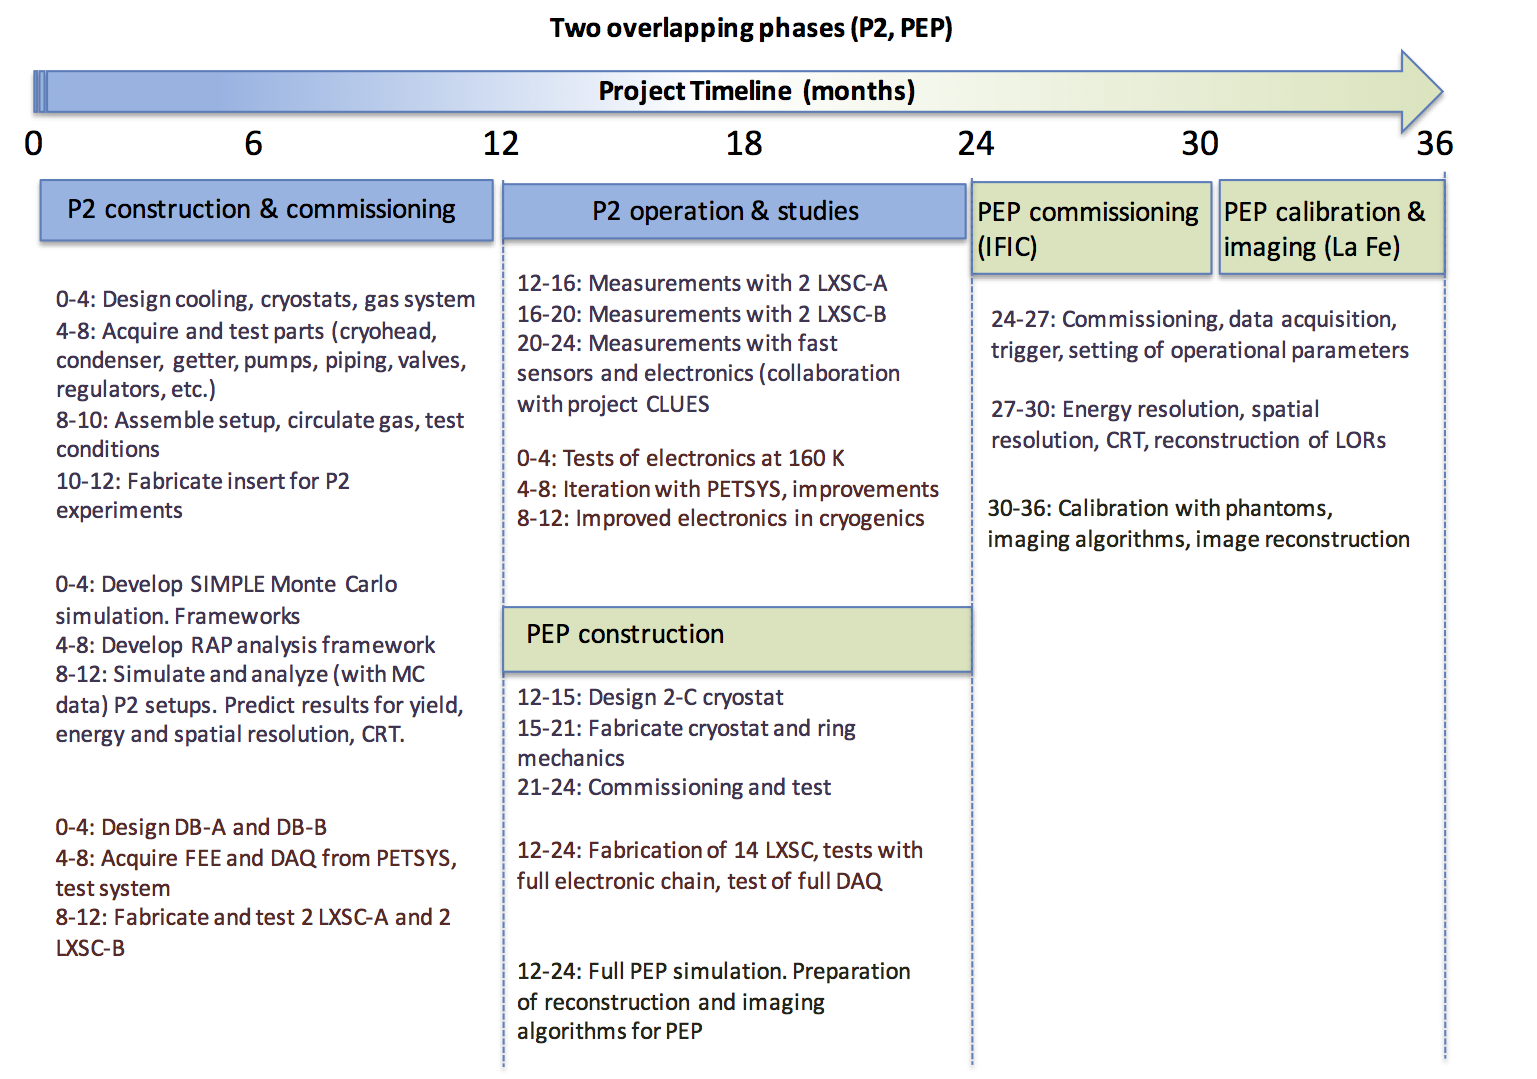
\includegraphics[scale=0.5]{img/Crono.png}
	\caption{\label{fig.Crono} Cronogram of the PETALO project.  }
\end{figure}

The work flow of the different projects has been detailed in the Methodology. Figure \ref{fig.Crono} shows a simplified cronogram to illustrate the development of the project.

\subsection*{Personal / Personnel}

%7. Si se solicita ayuda para la contratación de personal, justificación de su necesidad y descripción de las tareas que vaya a desarrollar.
\subsubsection*{Personnel resources and requirements of the DET subproject}

Subproject DET will be coordinated by prof. J. D\'iaz and will benefit from the support of the IFIC technical division and the NEXT technical group.

The proposed objectives need a full-time mechanical engineer with expertise in cryogenics to design and build P2, PEP and the gas system. The mechanical engineer will work during the first year in the construction of the P2 detector, and during the second year in the construction of the PEP detector. During the third year, he or she will be in charge of the installation of PEP at the hospital La Fe, and the safety analysis needed for the certification of the apparatus. In addition, he or she will work in the design of a large PETALO scanner, applying the experience and know-how acquired during the first two years of the project.

In addition, a post-doc is needed also for three years. The post-doc will work in the development of SIMPLE and RAP during the first year of the project, will be in charge of the operation and data taking of P2 and PEP (second and third year), will play a leading role in the data analysis of both detectors, and will collaborate with the IMG group in imaging reconstruction.

The DET subproject requires 2 years for the mechanical engineer and 2 years for the post-doc. The project will seek funding for the third year competing to the regular national and international calls for support technicians, Juan de la Cierva, Marie Curie, and/or funds from the Severo Ochoa grant at IFIC.

\subsubsection*{Personnel resources and requirements of the ASIC subproject}

The ASIC subproject is based in the expertise existing  at the I3M/UPV, which includes the to co-PIs, Prof. V. Herrero Bosch (VHB), Prof. Rafael Gadea (RG).
In addition the group has  one student  currently working with VHB.

The project requires an electronic engineer for two years. He or she will be in charge of the construction and testing of the DBs for P2 and PEP, the setting up and commissioning of the DAQ and the development of the slow controls. In addition, the engineer will work in the characterisation of the electronics in cryogenics conditions. He or she will be closely supervised for all the above tasks by VHB and RG.

\subsubsection*{Personnel resources and requirements of the IMG subproject}
 The IMG subproject includes an interdisciplinary team, lead by Dr. Irene Torres, a nuclear physicist with a Ph.D. in medical imaging.

 The project needs a post-doc for two years. He or she will play a leading role in the development of imaging algorithms, reconstruction and integration of image post-processing and the extraction of imaging biomarkers.

The post-doc background will be focused in the field of biomedical engineering and medical physics, specially in medical imaging acquisition technologies and in medical imaging processing. He or she will start developing imaging reconstruction algorithms (see the methodology section) during the second year of the project using Monte Carlo Data and will continue during the third year using PEP data. The post-doc will also work in the assessment of the imaging reconstruction capabilities of a large PETALO-TOF scanner.

%The tasks to be addressed by the Post-Doc will be under the frame of the integration of the PET solution with the NMR, the requirements of the new technology and the aspects of image reconstruction and processing. These will include:
% \begin{enumerate}
%\item Definition of MRI compatibility requirements and clinical spatial resolution.
%\item Study and modelling of image degradation phenomena LXSC-PET.
%\item Mathematical modelling of signals from PET detectors.
%\item Integration in the software of the user interface of the system.
%\item Development of hybrid image reconstruction methods for PET-MRI.
%\item Development of algorithms for the extraction of imaging biomarkers.
%\item Integration of imaging biomarkers analysis in user interface.
%\end{enumerate}

\subsubsection*{Personnel costs}
The total personnel costs are computed assuming a total cost of 40,000 \euro\ to the project per post-doc or engineer. The total number of post-doc (engineer) years is 8, resulting in a proposed personnel costs of 320,000 \euro.


\vspace{12pt}

\noindent\textbf{C.3. IMPACTO ESPERADO DE LOS RESULTADOS / EXPECTED IMPACT}

%C.3. IMPACTO ESPERADO DE LOS RESULTADOS 

The expected impact of this project is very large. A successful proof of concept of PETALO would open the way to the subsequent construction of clinical PETs. PETALO offers the possibility to build a full-body, high sensitivity, TOF capable scanner at a very competitive cost. 
%many advantages over conventional SSDs based devices, including a much better energy resolution, true 3D reconstruction that minimises parallax effects and the capability to handle Compton interactions, which are much better identified in the LXSC than in conventional SSDs. In addition, PETALO will be designed, from the beginning, as a fully compatible device with NMR, including both hardware components and the development of the imaging software. On top of the above, PETALO offers the potential of a breakthrough in TOF-PET technology. Last, but not least, the cost of the detection material (LXe) is much lower than the cost SSDs such as LSO and the cost of the SiPMs is decreasing exponentially. Therefore, by developing suitable front-end electronics and DAQ, PETALO could become a very economical PET solution, appropriated for a future large-scale (full-body) PET.

This project will also advance the field in several other aspects, including: a) a more detailed understanding of the physics of liquid xenon; b) the potential to develop electronics suitable to work at 160 K; a collaborative effort with project CLUES (group ICCUB) to advance the field in the area of ultra-fast detectors and electronics. In particular, this project will allow the application of such detectors and electronics to the study of the fast signals produced by scintillation and Cherenkov light in liquid xenon. 

Each subproject in this coordinated project contributes in a decisive way to the impact of PETALO. Subproject DET focuses in transferring the know-how developed at IFIC by basic science experiments such as NEXT to an application of enormous importance for public health. Subproject ASIC provides the expertise in sensors, front-end electronics, data acquisition and ASIC development. Subproject IMG will bring the necessary expertise in image reconstruction and will be in charge of transferring the PEP detector to the clinical environment. 

PETALO has already produced a patent request, and a number of other patents will certainly follow. The apparatus can be clearly commercialised, given its many advantages over conventional PETs. The diffusion of the results will proceed through publications in journals and participation in national and international conferences. Once the proof of concept is operational, the research team will work actively with companies to explore join ventures and possibilities of transferring to the industrial sector. 


\vspace{12pt}

\noindent\textbf{C.4. CAPACIDAD FORMATIVA DEL EQUIPO / TRAINING CAPABILITIES OF THE GROUP}
The PETALO project represents a unique opportunity for training students. 

\subsubsection*{Training Capabilities of the IFIC group}

The PI of the project has supervised  10 Ph.D. thesis during his career. The student will have the unique opportunity to work in the construction of P2 and PEP, commission and analysis the data produced by the apparatus, and later participate in the imaging analysis, in particular concerning the TOF capabilities. The development of the thesis would correspond to the tasks described in the plan presented for DET. 

%In particular, the plan of studies will include:
%
%\begin{enumerate}
%\item {\bf Study of the energy resolution using photoelectric events.} Photoelectric events are easily characterised in the LXSC, as single-site deposition events (unless conventional SSDs, the LXSC can separate multiple-site events to an expected resolution of a few mm). Then, the energy in the LXSC is measured by adding the signal of all the SiPMs. The energy resolution is obtained by fitting the photoelectric peak. The energy resolution of the LXSC6 will be measured as reference (an energy resolution of better than 3\% FWHM is expected). Then, the energy resolution of the LXSC2 will be measured. A resolution better than 5\% FWHM is expected.
%\item {\bf Study of the position resolution using photoelectric events.} To estimate the position resolution from data, we will use the LXSC6 which provides 2 redundant measurements of each coordinate. Then, if $\chi_1,\chi_2$~are redundant measurements of a given coordinate, and $\Delta \chi = \chi_2 - \chi_1$~is the difference between them, the $\Delta \chi$ distribution should have mean zero and standard deviation  
%$\delta \Delta \chi \sim \sqrt{2} \delta \chi$. To estimate the position resolution of LXSC2, one starts by validating the Monte Carlo simulation of the LXSC, by comparing data and Monte Carlo results for the LXSC6. After demonstrating that the Monte Carlo reproduces correctly the simulation measured with data for the LXSC6, one can use the Monte Carlo to estimate the position resolution of LXSC2. Position resolution in the range of 1-2 mm are expected. 
%\item {\bf Study of the time resolution using photoelectric events.} Coincidence Resolution Time (CRT) will be measured by comparing the time stamp provided by the two opposite LXSC cells. A CRT in the range of 200-250 ps is expected.
%\end{enumerate}
%
%In addition, a program of studies for Compton interactions (starting with Compton events that deposit their full energy in the cell and show a double-site deposition, will be carried out. The program will include the study of the energy, position and time resolution for double-site Compton events, the study of the resolution to separate double-site events, and the feasibility of using Compton kinematics to improve the resolution of the back projected tracks. 
%

\subsubsection*{Training Capabilities of the I3M-UPV group}
\par The research team has already directed 5 Doctoral Thesis and is being directing 2 more at the moment. Both members of the research team have long experience in graduate and post-graduate teaching since they work as Associate Professors in the Electronics Engineering Department of  the Polytechnic University of Valencia. The PETALO project may become a source for Ph.D. thesis, associated with the precise control of all the instrumental aspects needed to achieve a CRT below 100 ps. This goal is feasible for VUV-sensitive SiPMs, but will require a deep understanding of all the response of the SiPM and the ASIC. 

%The student will have which could serve as evaluation of alternative solutions for the front-end architecture. For instance a further reduction of the DAQ deadtime would be desirable in order to increase maximum event rate. The proposed solution in PETALO would increase ASIC complexity to an unaffordable level if deadtimes under 0.5 $\mu$s must be achieved. However a scheme based on deep analog FIFOs may lead to better solutions yet many issues related to noise, signal degradation etc should be first solved.
%\par A usual work plan for a Doctoral Thesis in microelectronics for front-end integration should cover a three years time span as follows:
%\begin{description}
%  \item[TASK 1 (6 Months)] Complementary training and State of the Art review. Depending on the proposal some specific training might be needed by the student. A mandatory review of the state of the art will help to focus on the problem.
%  \item[TASK 2 (2 Month)] Design Specifications. Selection of technology node and design tools.
%  \item[TASK 3 (3 Months)] High level modeling of analog and digital blocks. A set of high level modelling languages will be used in order to obtain functional detailed models of the different blocks.
%  \item[TASK 4 (4 Months)] Architectural Simulations based on previous models to determine design trade-offs
%  \item[TASK 5 (5 Months)] Analog design. All the analog blocks will be designed and validated in a multilevel simulation testbench using digital block models.
%  \item[TASK 6 (3 Months)] Digital design.
%  \item[TASK 7 (4 Months)] Layout design, Parasitics Extraction and Simulation. The effects of parasitics due to layout design are included in simulations and the whole system can be simulated as a final verification process before production.
%  \item[TASK 8 (1 Month)] Sign-off preparation and Foundry first iteration (Cross design rule check, bonding diagram and package selection)
%  \item[TASK 9 (4 Months)] Prototype test and characterization. A testbench (including a PCB carrier) must be designed in order to test the prototype. A test protocol must be defined and a final characterization data sheet produced.
%  \item[TASK 10 (4 Months)] Thesis writing and results publishing. Some of the preliminary results (especially those related to the analog design) can be published before depending on their scientific value.
%\end{description}

\subsubsection*{Training Capabilities of the GIBI230 group}
The Principal Investigator and the members of the research group form a multidisciplinary team including physicists, nuclear physicians and telecommunications engineers inside the Biomedical Imaging Research Group GIBI230. This research group has huge experience in the training of fellows belonging to several universities from the Spanish territory and also from abroad. Furthermore, the members of the research team have participated as teachers in several courses and seminars related to the project topic. 
The research team members have experience in training students of different backgrounds, such as Physics or Medicine and also Biomedical Engineering, being two of the members, former trainees of their Biomedical Engineering master’s thesis.
The research team and the training fellow will have enough resources and equipment available to properly develop the assigned task of the project in the Medical Imaging Clinical Area of the University and Polytechnic Hospital La Fe. 
This experience indicates that the research team has sufficient training capacity to assume the incorporation of training fellow who could finish the doctoral thesis within the period of the project. 


%Este apartado solo se rellenará si alguno de los subproyectos participantes solicita la inclusión del proyecto en la convocatoria de “Contratos predoctorales para la formación de doctores”. Dicha inclusión solo será posible en un número limitado de los proyectos aprobados.
%
%Para evaluar la capacidad formativa del equipo solicitante, se recomienda incluir:
%
%1. El plan de formación previsto.
%
%2. Relación de tesis realizadas o en curso (últimos 10 años) con indicación del subproyecto, nombre del doctorando, el título de tesis y la fecha de obtención del grado de doctor o de la fecha prevista de lectura de tesis.
%
%3. Breve descripción del desarrollo científico o profesional de los doctores egresados de los equipos de investigación de los subproyectos participantes.

%%%%%%%%%%%%%%%%%%%%%%%%%%%%%%%%%%%%%%%%%%%%%%%%%%%%%%%%%%%%%%%%%%%%%%%%%%%%%

\vspace{12pt}

\noindent\textbf{C.5. IMPLICACIONES ÉTICAS Y/O DE BIOSEGURIDAD/ETHICS AND SAFETY IMPLICATIONS}

This project foresees the installation of PEP as a pre-clinical PET at LaFe during the last semester of the third year of the project. The initial studies at LaFe will be carried out with phantoms, in order to calibrate the PET and to characterise its performance. Therefore, it is not foreseen that PEP is used with human patients during the development of this project. It follows that there are no relevant ethical issues. 
%All procedures for animal research conducted in this project will follow the current legislation and in particular, Law 32/2007, of 7th November, for the care of the animals on his farm, transport, experimentation and sacrifice, in Law 6/2013, of 11th June, amending Law 32/2007, of 7 November, for the care of the animals on his farm, transport, experimentation and sacrifice and in Royal Decree 53 / 2013, of 1th February , establishing the basic standards for the protection of animals used for experimental and other scientific purposes, including teaching.

%\subsubsection*{Safety regulations}
%In the Experimental Radiology Area IIS La Fe properly follow biosecurity controls established by Council of Agriculture, Livestock and Fisheries of Valencia. The responsible Biological Risk and Work Hazard of IIS La Fe must make an assessment of them and obtain a User Center Registration for the project.
%All personnel who could access the area should know the limitations and contraindications and comply with the safety standards.
%
%%Staff working with animals is informed of the risks inherent in the work performed, following the rules Work Hazard Prevention for workers of Experimental Radiology.
%%Health risks from work with experimental animals (excluding primates) are much lower than the risks from work with human patients. In any case, regulatory actions under the veterinary supervision must always be respected.
%
%\subsubsection*{Minimising cross-contamination}
%
%The head of the Department of Experimental Radiology, before start any exam and provide access to the animals for this study, must ensure that there are no other animal in the areas of common access.
%On no account, personal, animals or materials should access from the Experimental Radiology Area to the Animal Lab without the consent of the responsible veterinarian.
%It will seek to have ventilation systems for rooms with information about air changes / hour and pressure relative to the hallway and adjoining rooms.
%NMR room of the Experimental Radiology Area has a positive pressure gradient from the Animal Lab to the imaging space. 
%
%\subsubsection*{Personal}
%
%The technician necessary for the performance of the project must have an adequate preparation with the corresponding training Course for Animal Research Experimenter (at least Category B).
%
%\subsubsection*{Equipment}
%It is the responsibility of the principal investigator of the project along with the responsible of the Department of Experimental Radiology to ensure that the working conditions are appropriate and there is all necessary material for the study.
%The image material as well as anaesthesia must be previously identified and tested. It must be check the functioning of all the devices before starting the study.


\end{document}

